% ============================================================
% Multimodal Breast Cancer Molecular Subtyping Paper
% Target: Bioinformatics / IEEE JBHI / Briefings in Bioinformatics
% ============================================================
\documentclass[11pt,a4paper]{article}

% ---- Packages ----
\usepackage[utf8]{inputenc}
\usepackage[T1]{fontenc}
\usepackage{amsmath,amssymb}
\usepackage{graphicx}
\usepackage{booktabs}
\usepackage{multirow}
\usepackage{array}
\usepackage{caption}
\usepackage{subcaption}
\usepackage{float}
\usepackage{xcolor}
\usepackage{hyperref}
\usepackage[margin=2.5cm]{geometry}
\usepackage{setspace}
\usepackage{natbib}
\usepackage{enumitem}
\usepackage{tikz}
\usetikzlibrary{shapes.geometric, arrows.meta, positioning, fit, calc, backgrounds}

% ---- Custom colors ----
\definecolor{accentblue}{RGB}{31,119,180}
\definecolor{accentorange}{RGB}{255,127,14}
\definecolor{accentgreen}{RGB}{44,160,44}

% ---- Line spacing ----
\doublespacing

% ============================================================
\begin{document}

\title{%
  \textbf{Label-Space Mismatch Distorts Cross-Cohort Evaluation in \\
  Breast Cancer Molecular Subtyping}%
}

\author{Shuxing Liu\thanks{Shuxing Liu is with the Faculty of Medicine and Health Sciences, Universiti Sains Malaysia, Kubang Kerian, Kelantan, Malaysia (e-mail: liushuxing8888@student.usm.my).}\thanks{Corresponding author: Shuxing Liu (e-mail: liushuxing8888@student.usm.my).}}

\date{\today}

% Single-space the title block: the document-wide \doublespacing setting is
% applied to the manual line break in the title and leaves a conspicuous gap.
\begin{spacing}{1}
\maketitle
\end{spacing}

% ============================================================
\begin{abstract}
\noindent
\textbf{Background:} Cross-cohort evaluations can be misleading when datasets use different annotation standards. We assessed this problem in breast cancer molecular-subtype classification, where METABRIC labels include six classes and PAM50 annotations include five intrinsic subtypes.

\textbf{Methods:} The METABRIC multimodal analysis included 1,369 patients with aligned data, split into training (n=958), validation (n=205), and test (n=206) sets. External label-space analyses used mRNA classifiers on TCGA-BRCA (n=987) and GSE21653 (n=266). We compared uncorrected predictions with restriction to the five PAM50 classes and expectation-maximisation (EM) prior correction, without using target labels. We then harmonized a reduced three-layer space that both METABRIC and TCGA-BRCA carry (412-gene mRNA panel, 232-gene methylation panel, 10 shared clinical fields; TCGA n=694) and re-ran the modality ablation inside it, to test whether the multimodal advantage transfers.

\textbf{Results:} In this series, the annotation space, not the model, dominated reported cross-cohort performance. Uncorrected accuracy was 73.76\% on TCGA-BRCA, similar to 73.8\% on the METABRIC test set, and six-class macro F1 was 0.585 against 0.702 when scored over its five annotated classes. On GSE21653, uncorrected accuracy was 63.16\%. Restricting predictions to PAM50 classes and applying EM correction raised accuracy to 80.65\% on TCGA-BRCA and 74.06\% on GSE21653; these are changes in evaluation rules, not improvements in the learned representation. Within the harmonized space, the multimodal advantage did not transfer. Adding methylation was flat under cross-validation and lowered TCGA accuracy by 1.9 points; the harmonized clinical block raised held-out METABRIC test accuracy by 2.4 points but moved TCGA accuracy by 0.3 points or less; and no multimodal configuration differed significantly from mRNA alone (paired McNemar, $p=0.13$ to $1.00$). The 713-dimension flagship that performs best internally (75.92\% cross-validated) is not transportable, because 59 of its clinical dimensions are METABRIC-specific. Unconstrained EM assigned the absent claudin-low class a prior of 0.0751 on TCGA-BRCA, and no tested detector identified absent classes reliably across covariate and prior shift: re-scored under the standard empty-set convention, the original uncalibrated rule has the highest F1 (0.786) and exact-set match (0.550) of six tested, but its mean F1 on cohorts with a truly absent class falls from 0.995 to 0.543 at the highest covariate shift, while its calibrated replacements flag clean cohorts in 73 and 87 of 120 cases. Survival discrimination was similar across the external cohorts (C-index 0.577 and 0.584). In GSE20194 (n=278), the genomic panel did not significantly improve pCR prediction over clinical variables ($\Delta$AUC = +0.0045; 95\% CI, $-0.060$ to $+0.061$).

\textbf{Conclusions:} Cohort-level performance is not directly comparable when annotation standards define different label spaces, and the target cohort's allowed labels should be established before computing comparative metrics; in these experiments, unlabeled predictions alone did not identify the absent class. The same discipline applies to modality fusion: in the one cohort pair where the multimodal model could be evaluated under an identical input definition, its advantage was internal only.
\end{abstract}


\textbf{Keywords:} breast cancer, molecular subtyping, PAM50, label-space mismatch, label shift, cross-cohort evaluation, multimodal integration

% ============================================================
\section{Introduction}
\label{sec:intro}

Breast cancer is a heterogeneous disease characterized by distinct molecular subtypes that differ in gene expression patterns, clinical behavior, and treatment response \citep{perou2000molecular}. The PAM50 classification system defines five intrinsic subtypes: Luminal A, Luminal B, HER2-enriched, Basal-like, and Normal-like \citep{parker2009supervised}. Claudin-low is a separate designation based on additional markers \citep{prat2010phenotypic}. Accurate subtyping can inform treatment selection and prognosis assessment \citep{prat2014research}.

Current approaches to breast cancer subtyping predominantly rely on single data modalities. The Prosigna (PAM50) test uses only gene expression data \citep{parker2009supervised}, while clinical risk calculators such as Nottingham Prognostic Index use only clinicopathological features \citep{haybittle1982prognostic}. However, breast cancer biology is driven by the interplay of genomic, epigenomic, and clinical factors. DNA methylation patterns, for instance, play a crucial role in regulating gene expression in breast cancer \citep{pasculli2018epigenetics}, and clinical variables such as ER/PR/HER2 status carry independent prognostic information \citep{goldhirsch2013personalizing}.

Multimodal learning has emerged as a promising paradigm for cancer classification, with studies demonstrating that integrating multiple data types can improve prediction accuracy and biological understanding \citep{wang2014similarity, chaudhary2018deep, sharifinoghabi2019moli}. However, several challenges remain: (1) many multimodal approaches require large training datasets that are unavailable for rare cancer subtypes; (2) models trained on one profiling platform often fail to generalize to data from different platforms; and (3) the relative contributions of different modalities are poorly understood.

Label-shift methods provide established tools for estimating or correcting changes in class prevalence from unlabeled target predictions. These include black-box shift estimation, EM-based prior adjustment, regularized adaptation, calibration-aware estimation, and methods for open-set or generalized label shift \citep{lipton2018detecting,azizzadenesheli2019regularized,saerens2002adjusting,alexandari2020maximum,garg2020unified,garg2022open,tachetdescombes2020domain}. These methods address changes in class proportions within a specified label space. They do not by themselves establish that source and target annotation standards define the same set of classes. We examine that distinction in breast cancer molecular-subtype evaluation rather than proposing a new label-shift algorithm.

We use a multimodal METABRIC model as an internal reference and focus the cross-cohort analysis on its mRNA classifier, the feature block available across cohorts. The central question is whether apparent performance differences can be interpreted before reconciling the target cohort's annotation space. We quantify the effect of restricting predictions to the five PAM50 classes, separate that operation from prior correction, and test whether absent classes can be inferred from unlabeled predictions. Survival discrimination and multimodal feature attribution provide secondary analyses.

The analysis raised a question about a lower accuracy observed in one external cohort. The target cohort used PAM50 annotations, whereas the METABRIC model had six output classes, including claudin-low. Predictions assigned to a class excluded by the target annotation standard cannot be correct under that evaluation. Section~\ref{sec:labelspace} measures the effect of reconciling the label space and compares it with prior correction. It also evaluates whether the absent class can be identified from unlabeled target predictions.

Our key contributions are:
\begin{enumerate}[nosep]
  \item We quantify how a mismatch between the six-class training label space and the five-class PAM50 annotation space changes cross-cohort metrics, separately from prior correction (Section~\ref{sec:labelspace});
  \item Using the annotation-standard fact that claudin-low is not a PAM50 subtype, without target labels, we change accuracy from 73.76\% to 80.65\% on TCGA-BRCA and from 63.16\% to 74.06\% on GSE21653. These are evaluation-rule changes, not retraining gains;
  \item We show that the tested unlabeled-data procedures do not reliably identify the absent class. Unconstrained EM retains an estimated claudin-low prior of 0.0751 on TCGA-BRCA, and two tested detectors do not reliably recover the annotation space;
  \item We report a negative result for cross-modal attention fusion. Capacity sweeps, regularization, and self-supervised pretraining did not bring the tested architecture to the linear reference, and its internal gains did not transfer;
  \item A systematic evaluation of modality combinations, demonstrating that clinical + mRNA + methylation outperforms all five modalities, together with SHAP-based modality attribution and survival analysis confirming significant prognostic stratification.
\end{enumerate}

% ============================================================
\section{Methods}
\label{sec:methods}

\subsection{Data Collection and Preprocessing}
\label{sec:data}

\subsubsection{METABRIC Dataset}
The Molecular Taxonomy of Breast Cancer International Consortium (METABRIC) dataset \citep{curtis2012genomic} was used as the primary development cohort. The source cohort contained 1,974 patients with PAM50 annotations. The analysis set comprised 1,369 patients retained after aligning patient identifiers across the clinical, mRNA, copy-number, methylation, and mutation records used in preprocessing. The 1,369-patient analysis set was split into training, validation, and test subsets. Five-fold cross-validation estimates were computed within the training subset (n=958), not across the full aligned analysis set.

Clinical features were encoded from 22 categorical and continuous variables including age at diagnosis, tumor size, tumor stage, ER/PR/HER2 status, and treatment history. Categorical variables were one-hot encoded, and continuous variables were Z-score standardized, yielding 69 clinical feature dimensions. mRNA expression data were filtered to 412 genes (subset of the 488 available genes matching the TCGA gene panel), and DNA methylation comprised 232 CpG probes selected by variance ranking.

The analysis set was split into training (n=958, 70\%), validation (n=205, 15\%), and test (n=206, 15\%) sets using stratified random sampling to preserve subtype proportions. Class distribution in the training set: Luminal A (35.7\%), Luminal B (23.9\%), HER2-enriched (12.5\%), claudin-low (9.5\%), Basal-like (10.4\%), and Normal-like (7.9\%).

\subsubsection{TCGA-BRCA External Validation Dataset}
The Cancer Genome Atlas Breast Cancer (TCGA-BRCA) cohort \citep{cancer2012comprehensive} was used for external validation. From the Firehose Legacy study (1,108 patients), we obtained RNA-seq V2 expression data (1,100 samples) and PAM50 annotations (987 samples with 5 subtypes; claudin-low not annotated). Survival data were available for 966 patients with 133 death events (13.8\% event rate).

Gene expression was mapped from the 412-gene METABRIC panel using Entrez Gene IDs via the cBioPortal API. Within each platform, expression values were rank-transformed and normalized using the inverse normal CDF to achieve cross-platform comparability:
\begin{equation}
  x_{ij}^{\text{norm}} = \Phi^{-1}\left(\frac{\text{rank}(x_{ij})}{n_j + 1}\right)
  \label{eq:rank_norm}
\end{equation}
where $\Phi^{-1}$ is the inverse normal CDF and $n_j$ is the number of samples in platform $j$. This within-platform normalization preserves relative sample ordering while removing platform-specific distributional differences.

\subsubsection{GEO External Cohorts}
GSE21653 was obtained from the Gene Expression Omnibus (GEO; \url{https://www.ncbi.nlm.nih.gov/geo/query/acc.cgi?acc=GSE21653}). It comprises 266 tumors profiled on GPL570 (Affymetrix Human Genome U133 Plus 2.0), with PAM50 subtype calls and disease-free survival records. Of the 412 genes in the METABRIC panel, 369 mapped to this platform. When multiple probes mapped to one gene, the probe with the highest mean expression was retained. Expression values were normalized within the cohort using the rank-based procedure above.

GSE20194 was obtained from GEO (\url{https://www.ncbi.nlm.nih.gov/geo/query/acc.cgi?acc=GSE20194}) for the secondary pathological complete response (pCR) analysis. The cohort included 278 patients treated with neoadjuvant chemotherapy, of whom 56 achieved pCR and 222 had residual disease. The series was profiled on the Affymetrix Human Genome U133A platform (GPL96); 276 genes from the 412-gene panel mapped to this platform. The published pCR labels were used only as the outcome for this secondary analysis.

\subsection{Multimodal Feature Engineering}
\label{sec:features}

We engineered features from five modalities:
\begin{enumerate}[nosep]
  \item \textbf{Clinical} (69d): One-hot encoded categorical variables (e.g., ER status, HER2 status, tumor stage, surgery type, treatment history) with Z-score standardized continuous variables (age, tumor size, lymph node count, NPI).
  \item \textbf{mRNA expression} (412d): Microarray expression values for 412 genes, Z-score standardized.
  \item \textbf{Copy number alteration} (256d): Top 256 genes by variance from SNP 6.0 array, Z-score standardized.
  \item \textbf{DNA methylation} (232d): Beta values for 232 CpG probes selected by variance, Z-score standardized.
  \item \textbf{Somatic mutations} (173d): Binary indicators for 173 genes with at least one mutation in the cohort.
\end{enumerate}

Total feature dimensions across all modalities: $69 + 412 + 256 + 232 + 173 = 1{,}142$.

\subsection{Model Development}
\label{sec:models}

\subsubsection{Logistic Regression}
Multinomial logistic regression was chosen as the primary classifier due to its strong performance on small-sample, high-dimensional data and inherent interpretability. The model uses the softmax function:
\begin{equation}
  P(y = k \mid \mathbf{x}) = \frac{\exp(\mathbf{w}_k^\top \mathbf{x} + b_k)}{\sum_{j=1}^{K} \exp(\mathbf{w}_j^\top \mathbf{x} + b_j)}
  \label{eq:softmax}
\end{equation}
with $L_2$ regularization controlled by parameter $C$. We evaluated $C \in \{0.001, 0.01, 0.1, 1.0, 10.0\}$, with $C = 0.01$ selected by cross-validation. Estimators were implemented with scikit-learn \citep{pedregosa2011scikit}.

\subsubsection{Comparison Models}
We compared logistic-regression regularization variants and a sigmoid-calibrated model with Random Forest (300 trees), XGBoost, LightGBM, CatBoost, Extra Trees, soft-vote ensembles, and Transformer variants. The Transformer model used five modality-specific linear projections feeding into a two-layer encoder (d\_model=64, four attention heads) with a classification head (174K parameters).

\subsubsection{Ensemble and Cascade Methods}
We explored: (1) soft-vote ensemble of LogReg + GBDT + XGBoost; (2) a two-stage cascade where LogReg classifies high-confidence samples and a Transformer handles low-confidence samples; and (3) a Guided Transformer where LogReg probability outputs serve as a soft prompt token for cross-modal attention.

\subsection{Evaluation Protocol}
\label{sec:eval}

\subsubsection{Classification Metrics}
Primary metrics: accuracy and macro-averaged F1-score. Secondary metrics: per-class precision, recall, and F1-score. Statistical significance of model differences was assessed using McNemar's test on the held-out test set.

\subsubsection{Survival Analysis}
Predicted subtype probabilities were used as covariates in a Cox proportional hazards model:
\begin{equation}
  h(t) = h_0(t) \exp\left(\sum_{k=1}^{K-1} \beta_k \hat{p}_k\right)
  \label{eq:cox}
\end{equation}
where $\hat{p}_k$ is the predicted probability for subtype $k$ (Luminal A as reference), and $h_0(t)$ is the baseline hazard. Discrimination was assessed using the concordance index (C-Index) at 3-year, 5-year, and 10-year time horizons. Kaplan-Meier survival curves were compared using the log-rank test.

\subsubsection{Interpretability Analysis}
SHAP (SHapley Additive exPlanations) \citep{lundberg2017unified} with the LinearExplainer was used to quantify feature importance. Modality contribution was computed as the mean absolute SHAP value aggregated across all features within each modality. The analysis was performed on a 300-sample subset of the training data.

\subsubsection{Label-Space Reconciliation and Prior Correction}
\label{sec:methods_shift}

Because the training cohort carries six classes and the external cohorts carry five, the
classifier's output space must be reconciled before any accuracy is computed. We define a
\emph{label-space mask} $m \in \{0,1\}^K$ with $m_k = 0$ for any class $k$ that the target
cohort's annotation standard cannot emit. For PAM50-annotated cohorts this mask is fixed by the
annotation standard alone. Claudin-low is not one of the five PAM50 intrinsic subtypes
\citep{parker2009supervised}, so the mask is \emph{independent of the target labels}. This
distinction is load-bearing and we state it explicitly: deriving the mask from
$\mathrm{unique}(y_{\text{target}})$ would leak the labels and inflate the result, so every
number reported in Section~\ref{sec:labelspace} uses the hard-coded annotation mask.

We compare four estimators within each target cohort. They share the same fitted classifier and
feature set within that cohort. TCGA-BRCA uses all 412 mapped genes. GSE21653 uses the 369 genes
mapped to GPL570, with the source classifier refitted on the corresponding METABRIC columns:

\begin{enumerate}[nosep]
  \item \textbf{base}: $\arg\max_k p_k$, with no reconciliation (the conventional protocol);
  \item \textbf{mask\_only}: zero the masked columns and renormalise;
  \item \textbf{em\_pam50}: expectation-maximisation prior correction \citep{saerens2002adjusting}
        over the full $K$-class space, with masked columns fixed at zero throughout;
  \item \textbf{em\_full}: the same EM procedure with \emph{no} mask, meaning it receives no label-space
        knowledge whatsoever.
\end{enumerate}

The source prior is the METABRIC training composition. EM updates the target probabilities and
class priors as follows:
\begin{align*}
p_k^{(t+1)}(x) &\propto p_k^{(t)}(x)\, \pi_k^{(t)} / \pi_k^{(0)}, \\
\pi^{(t+1)} &= \mathbb{E}_x[p^{(t+1)}(x)].
\end{align*}
Iterations stop when the prior changes by less than $10^{-6}$. The contrast between
\textbf{em\_pam50} and \textbf{em\_full} isolates the value of the label-space fact. Both use
identical unlabelled target predictions, but only one is given the structurally impossible classes.

Gains are reported with a paired bootstrap ($n_{\text{iter}} = 2000$, resampling target samples
and recomputing both endpoints), and a split-half transductive check confirms the correction
does not depend on how the target is partitioned.

\subsubsection{Controlled Simulation of Mismatch}
\label{sec:methods_sim}

To separate the contributions of label-space mismatch from ordinary prior shift we simulate
targets under a full factorial design: label-space mismatch $n_{\text{absent}} \in \{0,1,2\}$,
covariate shift $\in \{0.0, 0.4, 0.8\}$, and prior shift $\in \{\text{false}, \text{true}\}$,
with 20 seeds per cell and $n_{\text{target}} = 1000$. Absent classes are the two rarest in the
source prior; a class is treated as absent when its target prevalence falls below
$\tau_{\text{absent}} = 0.02$ or below $\tau_{\text{ratio}} = 0.10$ of its source prevalence.
Each cell reports accuracy with no correction, with an oracle label-space mask, and with a mask
estimated from the target.

\subsubsection{Geometric Absence Detection}
\label{sec:methods_detector}

We also asked whether the absent class could be identified from unlabelled predictions alone,
without being told. We built a detector on the geometry of the target probability simplex: for
candidate absent set $S$, measure the ratio of observed mass to source-expected mass on the
columns in $S$, and flag $S$ when that ratio exceeds a threshold $\tau$. The threshold was
calibrated on null data (no truly absent class) at level $\alpha = 0.05$, taking the 95th
percentile of the maximum ratio statistic under the null. This calibration is what makes the
detector a fair test rather than a tuned one: $\tau^\ast$ is chosen so that a cohort with no
absent class is flagged at most 5\% of the time.

\subsubsection{Generative Model-Selection Detection}
\label{sec:methods_lrt}

Because a hand-calibrated threshold is the obvious objection to the detector above, we also tested a
mechanism that sets no threshold at all. Here the target sample is modelled as
$p(x) = \sum_{k \in M} \pi_k \, \mathcal{N}(x ; \mu_k, \Sigma)$, with the component means and the
shared covariance estimated from the \emph{source} labels and the mixture weights $\pi$ fitted on
the unlabelled \emph{target} by expectation-maximisation over an allowed label space $M$. Candidate
label spaces are all subsets of size 4, 5, or 6. This includes every configuration with zero, one, or two
absent classes. The winner is the subset minimising the Bayesian information criterion
$\mathrm{BIC} = -2\log L + (|M| - 1)\log n$, so the complexity penalty, rather than a tuning
constant, is what controls the trade-off; predictions are formed on a 40-component PCA projection
of the standardised features. No target labels are used at any point.

% ============================================================
\section{Results}
\label{sec:results}

\subsection{Modality Selection Reveals Optimal Feature Combination}
\label{sec:modality}

Systematic evaluation of modality combinations (Table~\ref{tab:modality_ablation}) revealed that adding more modalities did not always improve performance. The clinical + mRNA + methylation model (713 dimensions) achieved 79.0\% validation accuracy, 3.4 percentage points above the full five-modality model (75.6\%). In cross-validation, adding CNA alone or mutation alone to the selected three-modality model reduced accuracy by 2.3 and 2.0 points, respectively. The full five-modality model scored 72.4\%, 2.9 points below the selected model.

\begin{table}[H]
\centering
\caption{Modality-combination ablation on the METABRIC validation set (n=205). Five-fold cross-validation results use the training subset (n=958). The clinical + mRNA + methylation model exceeds the all-modality model by 3.4 percentage points on the validation split.}
\label{tab:modality_ablation}
\begin{tabular}{lcrc}
\toprule
\textbf{Modality Combination} & \textbf{Dim} & \textbf{Val Acc (\%)} & \textbf{5-fold CV (\%)} \\
\midrule
Clinical only & 69 & 63.9 & 64.1 $\pm$ 2.7 \\
mRNA only & 412 & 74.6 & 73.8 $\pm$ 1.6 \\
Methylation only & 232 & 56.6 & 54.7 $\pm$ 2.4 \\
\midrule
Clinical + mRNA & 481 & 75.6 & 74.5 $\pm$ 1.9 \\
Clinical + Methylation & 301 & 68.3 & 65.7 $\pm$ 1.9 \\
mRNA + Methylation & 644 & 74.6 & 73.1 $\pm$ 2.6 \\
\midrule
\textbf{Clinical + mRNA + Methylation} & \textbf{713} & \textbf{79.0} & \textbf{75.3 $\pm$ 2.6} \\
+ CNA (4 modalities) & 969 & 75.6 & 73.0 $\pm$ 1.8 \\
+ Mutation (4 modalities) & 886 & 77.6 & 73.3 $\pm$ 2.0 \\
All 5 modalities & 1142 & 75.6 & 72.4 $\pm$ 2.0 \\
\bottomrule
\end{tabular}
\vspace{2pt}
\par\footnotesize Validation accuracy was computed on the held-out split using a scaler fit on the training split.
\end{table}

\begin{figure}[htbp]
\centering
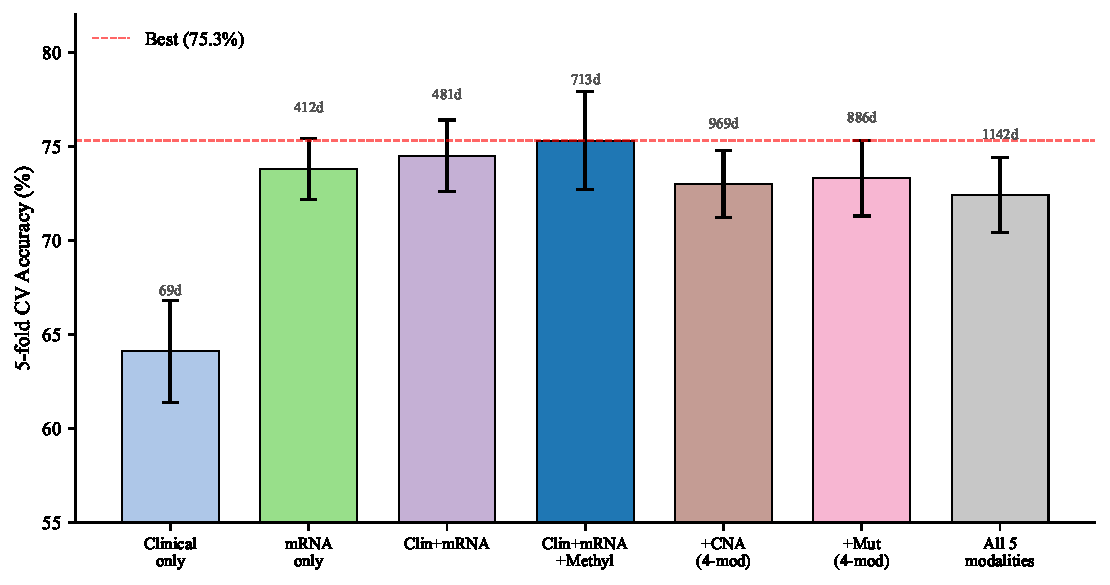
\includegraphics[width=0.85\textwidth]{figures/fig1_modality_ablation.pdf}
\caption{Modality combination ablation, with feature dimensionality annotated above each bar.
The 3-modality combination (713 dimensions) is the optimum; adding copy-number or mutation blocks
lowers cross-validated accuracy by 2.3 and 2.0 points respectively despite the larger input.}
\label{fig:modality_ablation}
\end{figure}

\subsection{Model Comparison and Hyperparameter Sensitivity}
\label{sec:model_comparison}

Logistic regression with $C = 0.01$ achieved the highest 5-fold cross-validation accuracy (75.3\% $\pm$ 2.6\%) among the evaluated models (Table~\ref{tab:model_comparison}; Figure~\ref{fig:model_comparison}). Ensemble methods and Transformer architectures did not surpass the linear model in this comparison. The best Transformer variant achieved 68.5\% cross-validated accuracy.

\begin{table}[H]
\centering
\caption{Model comparison using five-fold cross-validation on the METABRIC training subset (n=958). Models use the selected clinical + mRNA + methylation feature set (713 dimensions), unless otherwise stated.}
\label{tab:model_comparison}
\begin{tabular}{lcc}
\toprule
\textbf{Model} & \textbf{CV Accuracy (\%)} & \textbf{Std} \\
\midrule
Logistic Regression ($C=0.01$) & \textbf{75.3} & \textbf{2.6} \\
Logistic Regression ($C=0.1$) & 74.1 & 2.3 \\
Logistic Regression ($C=1.0$) & 72.9 & 2.1 \\
Calibrated LogReg (sigmoid) & 74.4 & 2.1 \\
Random Forest (300 trees) & 72.4 & 2.4 \\
XGBoost & 72.0 & 3.3 \\
LightGBM & 71.0 & 3.1 \\
CatBoost & 73.9 & 2.7 \\
Extra Trees & 71.3 & 1.7 \\
Soft-vote Ensemble (LR+GB+XGB) & 72.6 & 2.8 \\
Transformer (d=64, 2-layer) & 68.5 & 1.8 \\
Guided Transformer (LR prompt) & 74.0 & 1.0 \\
LR $\rightarrow$ Guided TF Cascade & 76.2 & 2.0 \\
\bottomrule
\end{tabular}
\end{table}

\begin{figure}[htbp]
\centering
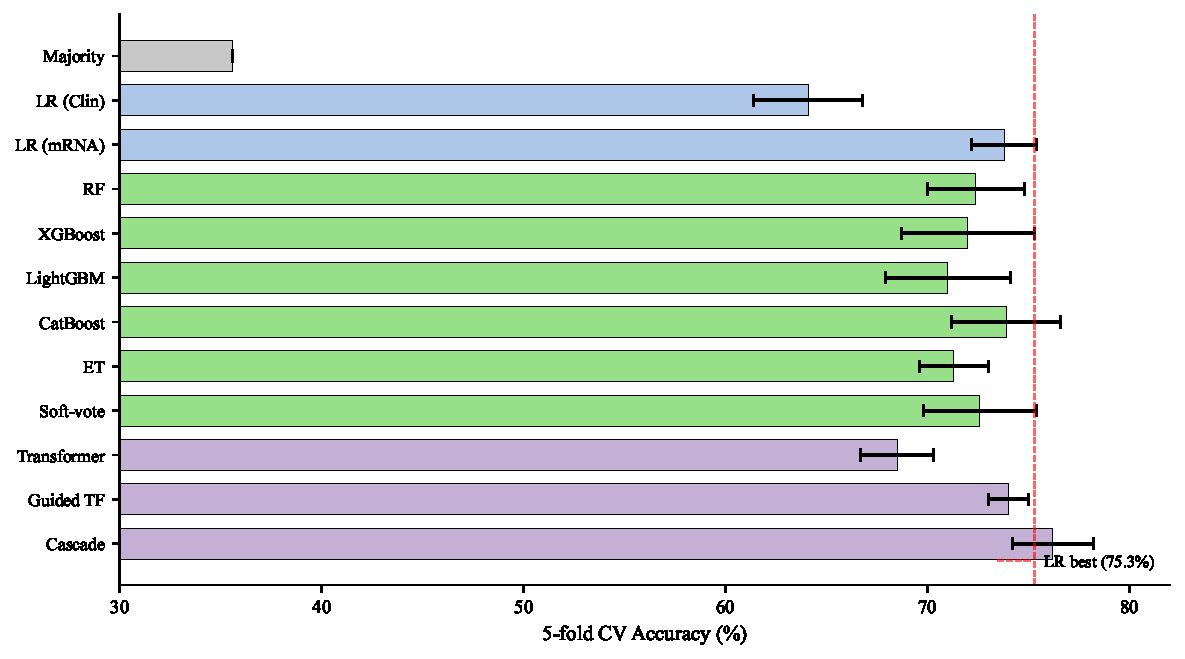
\includegraphics[width=0.9\textwidth]{figures/fig5_model_comparison.pdf}
\caption{Five-fold cross-validation model comparison on the selected METABRIC feature set.}
\label{fig:model_comparison}
\end{figure}

The cascade approach (LogReg $\rightarrow$ Guided Transformer) achieved a CV accuracy of 76.2\%, compared with 75.3\% for logistic regression alone. This 0.9-point difference was within the standard deviation of both estimates. On TCGA-BRCA, the 412-gene logistic-regression reference reached 73.8\%, whereas the unguided Transformer reached 66.1\% (Table~\ref{tab:route_a}).

\subsection{Feature Selection Identifies a Reduced Gene Set}
\label{sec:feature_selection}

ANOVA-based feature selection showed that mRNA-only cross-validated accuracy plateaued at approximately 200 genes (74.5\%). The top discriminating genes included \textit{ACOT4} (F=130.8), \textit{A2ML1} (F=102.0), and \textit{ABAT} (F=98.5). With clinical and methylation features, 200 mRNA genes achieved 75.5\% cross-validated accuracy, similar to the full 412-gene panel (Supplementary Table S3).

\subsection{Internal Validation Confirms Robust Performance}
\label{sec:internal}

On the held-out METABRIC test set (n=206), the 3-modality logistic regression achieved 73.8\% accuracy and 0.683 macro F1-score (Table~\ref{tab:internal_per_class}). The model showed strong performance for Luminal A (F1=0.768), Luminal B (F1=0.796), and HER2-enriched (F1=0.755) subtypes, with lower performance for Normal-like (F1=0.417) which had the smallest sample size (n=16).

\begin{table}[H]
\centering
\caption{Per-class classification metrics on the METABRIC test set (n=206).}
\label{tab:internal_per_class}
\begin{tabular}{lcccc}
\toprule
\textbf{Subtype} & \textbf{Precision} & \textbf{Recall} & \textbf{F1-score} & \textbf{Support} \\
\midrule
Luminal A & 0.700 & 0.851 & 0.768 & 74 \\
Luminal B & 0.812 & 0.780 & 0.796 & 50 \\
HER2-enriched & 0.741 & 0.769 & 0.755 & 26 \\
Claudin-low & 0.733 & 0.579 & 0.647 & 19 \\
Basal-like & 0.778 & 0.667 & 0.718 & 21 \\
Normal-like & 0.625 & 0.312 & 0.417 & 16 \\
\midrule
\textbf{Macro avg} & \textbf{0.732} & \textbf{0.660} & \textbf{0.683} & 206 \\
Weighted avg & 0.738 & 0.738 & 0.730 & 206 \\
\bottomrule
\end{tabular}
\end{table}

Confusion analysis (Figure~\ref{fig:confusion}) revealed that Luminal A/Luminal B misclassification is the primary error source: 9.5\% of Luminal A samples were predicted as Luminal B, and 22.0\% of Luminal B samples were predicted as Luminal A. This reflects the biological similarity between these two subtypes, which share ER-positive status and differ primarily in proliferation rate \citep{prat2014research}. The largest single error rate is on Normal-like, 62.5\% of which is predicted as Luminal A (recall 0.312); with only 16 test samples this estimate is correspondingly imprecise.

\begin{figure}[htbp]
\centering
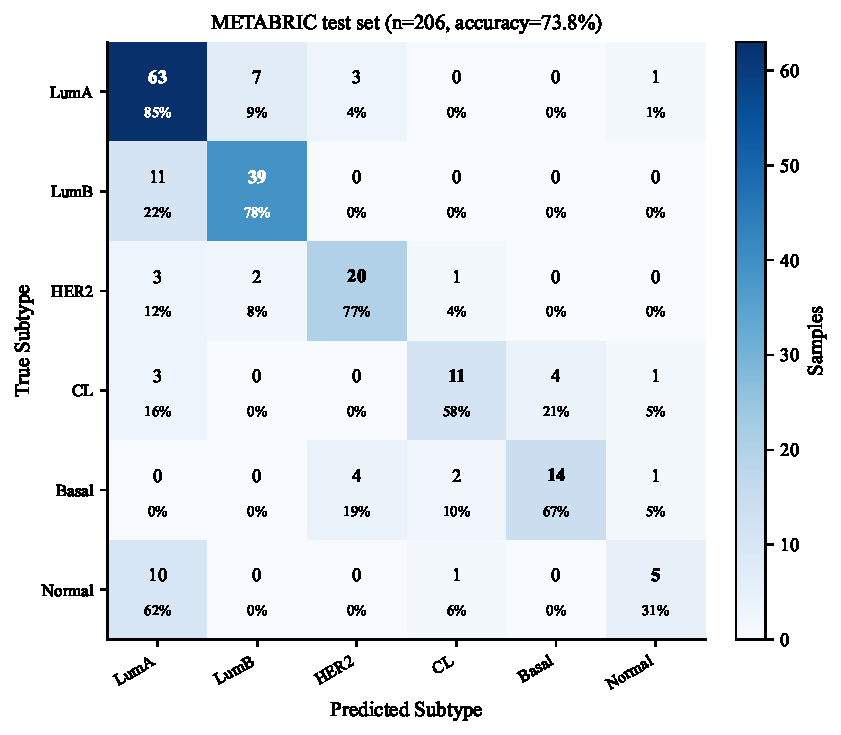
\includegraphics[width=0.85\textwidth]{figures/fig2_confusion_metabric.pdf}
\caption{Confusion matrix for the six-class PAM50 prediction task on the held-out METABRIC test set (n=206) for the 3-modality logistic regression (Clinical$+$mRNA$+$Methylation, 713 dimensions; accuracy 73.8\%). Cell values are predicted counts with row percentages. Luminal A/Luminal B confusion dominates the error budget.}
\label{fig:confusion}
\end{figure}

\subsection{External Validation Across Distinct Cohorts}
\label{sec:external}

The 412-gene mRNA-only model with within-platform rank normalization achieved 73.8\% accuracy on TCGA-BRCA (n=987, Figure~\ref{fig:tcga}), similar to its 73.8\% accuracy on the held-out METABRIC test set. The 69-dimension METABRIC clinical block has no direct counterpart in TCGA-BRCA: its NPI, GRADE, INTCLUST, and THREEGENE fields are METABRIC-specific, so the three-modality model cannot be evaluated on an identically defined input. A \emph{reduced} three-layer space that both cohorts share can be built, however, and Section~\ref{sec:external_multimodal} uses it to test whether the multimodal advantage survives external validation at all. The survival C-index was 0.577 ($p = 0.047$, log-rank test).

\begin{table}[H]
\centering
\caption{Per-class classification metrics on TCGA-BRCA external validation (n=987, 5 subtypes).}
\label{tab:tcga_per_class}
\begin{tabular}{lcccc}
\toprule
\textbf{Subtype} & \textbf{Precision} & \textbf{Recall} & \textbf{F1-score} & \textbf{Support} \\
\midrule
Luminal A & 0.904 & 0.749 & 0.819 & 502 \\
Luminal B & 0.600 & 0.709 & 0.650 & 199 \\
HER2-enriched & 0.667 & 0.846 & 0.746 & 78 \\
Basal-like & 0.978 & 0.762 & 0.856 & 172 \\
Normal-like & 0.500 & 0.389 & 0.438 & 36 \\
\bottomrule
\end{tabular}
\end{table}

\begin{table}[H]
\centering
\caption{Raw confusion matrix for TCGA-BRCA external validation (n=987), rows true and columns
predicted. Claudin-low appears as a predicted column but not as a true row because TCGA-BRCA
carries no claudin-low annotations: all 75 samples the model places there are necessarily errors.
Basal-like $\rightarrow$ claudin-low (38 samples) is the single largest off-diagonal block.}
\label{tab:tcga_confusion}
\begin{tabular}{lcccccc}
\toprule
\textbf{True $\backslash$ Pred} & \textbf{LumA} & \textbf{LumB} & \textbf{Her2} & \textbf{CL} & \textbf{Basal} & \textbf{Normal} \\
\midrule
Luminal A      & \textbf{376} & 87 & 10 & 15 & 0   & 14 \\
Luminal B      & 37 & \textbf{141} & 18 & 3  & 0   & 0  \\
HER2-enriched  & 2  & 5  & \textbf{66} & 3  & 2   & 0  \\
Basal-like     & 0  & 0  & 3  & 38 & \textbf{131} & 0  \\
Normal-like    & 1  & 2  & 2  & 16 & 1   & \textbf{14} \\
\midrule
\textbf{Predicted total} & 416 & 235 & 99 & \textbf{75} & 134 & 28 \\
\bottomrule
\end{tabular}
\end{table}

Macro F1 depends on the set of classes included in the average. We report it over the six-class
label space used for training. METABRIC contains all six classes and has macro F1 0.683. TCGA
contains five PAM50 classes, so claudin-low contributes an F1 of zero and the six-class average
is 0.585. Averaging the same predictions over the five PAM50 classes gives macro F1
\textbf{0.702}. This 0.117 difference is caused by the metric's class set; it does not represent
a change in predictions. Separately, the classifier predicted claudin-low for 75 TCGA samples
(7.6\%). Those predictions were errors and included 22.1\% of basal-like and 44.4\% of
Normal-like samples. TCGA also had a higher Luminal A prevalence than METABRIC (50.9\% versus
36\%) and only 36 Normal-like samples, of which 14 were correctly classified.

\begin{figure}[htbp]
\centering
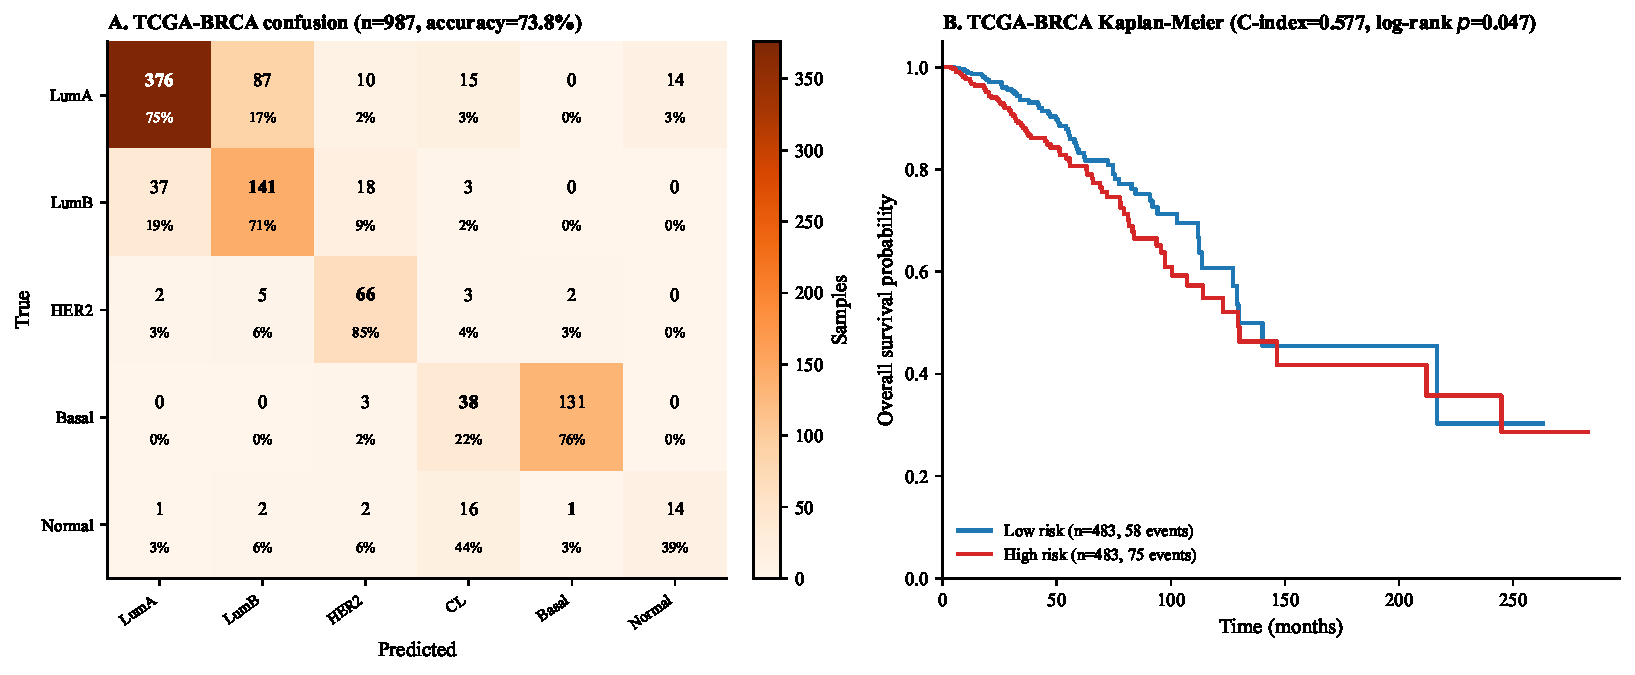
\includegraphics[width=0.85\textwidth]{figures/fig3_tcga_results.pdf}
\caption{External validation on TCGA-BRCA (n=987). The within-platform rank-normalized
mRNA model reaches 73.8\% accuracy and a survival C-index of 0.577 ($p=0.047$).}
\label{fig:tcga}
\end{figure}

\subsection{The Multimodal Advantage Does Not Survive External Validation}
\label{sec:external_multimodal}

The three-modality result in Section~\ref{sec:modality} was established on a single cohort. To
test whether it generalizes, we built a reduced space that METABRIC and TCGA-BRCA both carry and
re-ran the modality ablation inside it. Three layers were harmonized. mRNA uses the same 412-gene
panel, matched by symbol on both platforms (all 412 present; 10 are invariant on TCGA and were
assigned the neutral score). Methylation uses the 232-gene METABRIC panel, which is already
gene-level because the METABRIC preprocessing reduced probes to genes by variance; the
corresponding TCGA-BRCA HM450 gene-level values were retrieved from cBioPortal, and 209 of the
232 genes carry measurements (23 are absent from the array). Clinical uses the 10 fields present
in both schemas: age, pathologic stage, ER, PR, and HER2 status, and menopausal state. Every
continuous feature was rank-transformed to normal scores \emph{within its own cohort}, a
label-free operation, so no target labels were used at any point. Requiring all three layers plus
an annotated subtype leaves 694 TCGA-BRCA patients across the five PAM50 classes; claudin-low is
absent, as in the n=987 cohort.

Table~\ref{tab:multimodal_external} reports the ablation in this space. The pattern reverses. Adding
methylation produces no cross-validated gain on METABRIC (72.91\% for mRNA alone versus 72.91\% for
mRNA plus methylation) and lowers TCGA accuracy by 1.9 points, from 80.55\% to 78.67\%. Adding the
harmonized clinical block raises METABRIC cross-validated accuracy by 0.5 points and the held-out
METABRIC test score by 2.4 points, but moves TCGA accuracy by only 0.3 points in the unrestricted
setting and $-0.14$ points under the five-class restriction. No multimodal configuration differs
significantly from mRNA alone (paired McNemar, $p = 0.13$ to $1.00$), and the confidence intervals
overlap almost completely.

The two internal blocks move in opposite directions from their external counterparts, which is the
distinction Section~\ref{sec:labelspace} draws. On METABRIC the harmonized tri-modal model reaches
73.17\% cross-validated accuracy, while the original 713-dimension flagship reaches 75.92\%. That
2.75-point gap is attributable to the 59 clinical dimensions that exist only in METABRIC (NPI,
GRADE, INTCLUST membership, THREEGENE proliferation class, and cohort indicator); those fields are
not available in the target cohort, so the model that performs best internally is precisely the one
that cannot be transported. Conversely, the harmonized model's higher absolute TCGA accuracy
(80.55\% versus the published 73.76\%) reflects the label-space restriction, not better prediction:
under the five-class restriction the 64 samples the mRNA model sends to the absent claudin-low
column are reallocated to in-space classes, which is the same evaluation-rule change quantified
earlier.

We report this as a negative result about modality fusion, not as a failure of the pipeline. The
consistent finding across Sections~\ref{sec:route_a}--\ref{sec:route_a_multicohort} is that
additional modalities and additional architectural capacity raise internal cross-validated scores
while leaving or worsening external accuracy. The one intervention that improved external
performance was correcting the label space, not adding features.

\begin{table}[H]
\centering
\caption{Modality ablation in the harmonized three-layer space shared by METABRIC and TCGA-BRCA.
CV is five-fold cross-validated accuracy on pooled METABRIC train+val (n=1{,}163). TCGA accuracy
is on n=694 patients annotated with one of the five PAM50 classes present in that cohort; the
95\% CI is a bootstrap over patients. The McNemar column is a paired test against mRNA alone.
The final row is the original 713-dimension model, shown for reference: its clinical block
includes METABRIC-specific fields and has no external counterpart.}
\label{tab:multimodal_external}
\begin{tabular}{lcccccc}
\toprule
\textbf{Configuration} & \textbf{Dims} & \textbf{METABRIC CV} & \textbf{METABRIC test} &
\textbf{TCGA} & \textbf{TCGA macro F1} & \textbf{$p$} \\
\midrule
mRNA                       & 412 & 72.91 & 72.82 & \textbf{80.55} & 0.768 & --- \\
mRNA + clinical            & 422 & 73.43 & \textbf{75.24} & 80.40 & \textbf{0.774} & 1.00 \\
mRNA + methylation         & 644 & 72.91 & 72.33 & 78.67 & 0.747 & 0.13 \\
clinical + mRNA + methylation & 654 & 73.17 & 74.76 & 79.11 & 0.760 & 0.30 \\
\midrule
\emph{original flagship}   & \emph{713} & \emph{75.92} & \emph{73.79} & \emph{n/a} & \emph{n/a} & \emph{---} \\
\bottomrule
\end{tabular}
\end{table}

\begin{table}[H]
\centering
\caption{Bootstrap 95\% confidence intervals for the harmonized external evaluation (TCGA-BRCA,
n=694). Intervals overlap across all four configurations in both metrics.}
\label{tab:multimodal_ci}
\begin{tabular}{lcc}
\toprule
\textbf{Configuration} & \textbf{TCGA accuracy} & \textbf{TCGA macro F1} \\
\midrule
mRNA                       & 0.775--0.834 & 0.725--0.808 \\
mRNA + clinical            & 0.774--0.833 & 0.731--0.814 \\
mRNA + methylation         & 0.755--0.817 & 0.703--0.786 \\
clinical + mRNA + methylation & 0.759--0.820 & 0.717--0.798 \\
\bottomrule
\end{tabular}
\end{table}

\begin{figure}[htbp]
\centering
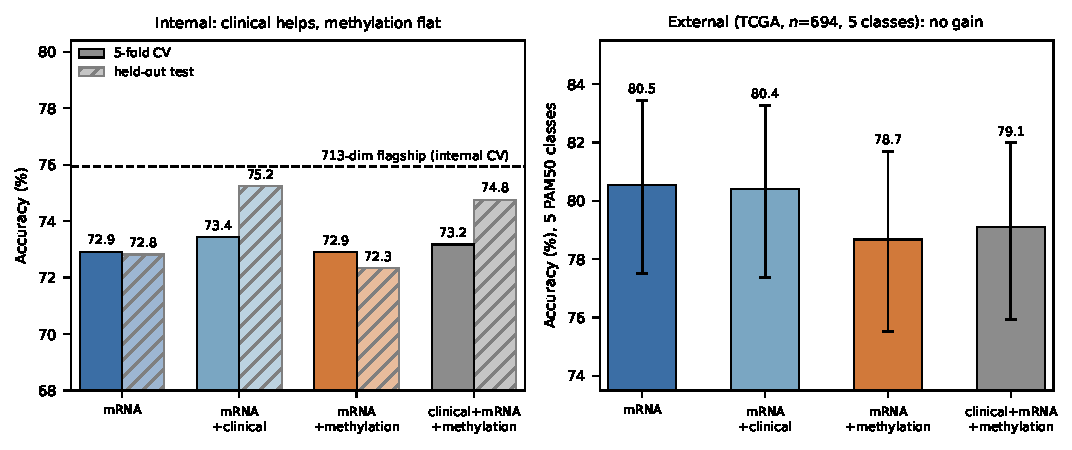
\includegraphics[width=0.95\textwidth]{figures/figJ_multimodal_external.pdf}
\caption{Internal and external behaviour of each modality configuration in the harmonized space.
Left: METABRIC cross-validated (solid) and held-out test (hatched) accuracy rise when the
harmonized clinical block is added, and methylation is flat. Right: on TCGA-BRCA, scored over the
five PAM50 classes present in that cohort, the same configurations are statistically
indistinguishable and methylation is the worst; error bars are bootstrap 95\% confidence intervals
over the 694 patients. The unrestricted six-class TCGA accuracy for mRNA alone is 73.34\%, the
same quantity plotted in Figure~\ref{fig:tcga} for the larger n=987 cohort. The dashed line marks the original 713-dimension
flagship's internal cross-validated accuracy; the 2.75-point gap to the harmonized tri-modal model
is contributed by METABRIC-only clinical fields that the target cohort does not carry.}
\label{fig:multimodal_external}
\end{figure}

\subsection{Label-Space Reconciliation Changes Cross-Cohort Evaluation}
\label{sec:labelspace}

Uncorrected accuracy on TCGA-BRCA (73.76\%) was similar to that on the METABRIC test set
(73.8\%), whereas accuracy on GSE21653 was lower (63.16\%). These observations do not support
a general claim that label-space mismatch explains every cross-cohort accuracy difference.
However, both external cohorts use PAM50 annotations, whose five intrinsic subtypes exclude
claudin-low, whereas the METABRIC classifier was trained on six classes. We therefore measured
how explicitly reconciling the label space changes the reported metrics, separately from prior
correction, without attributing all residual differences to annotation mismatch.

Predictions assigned to a class excluded by the target's annotation standard are necessarily
counted as errors under that standard. In TCGA, the model assigned 75 samples (7.6\%) to
claudin-low. These predictions included 22.1\% of basal-like and 44.4\% of Normal-like samples.
The resulting recall changes depend on which classes the model confuses with claudin-low.

\subsubsection{Effect of Label-Space Reconciliation and Prior Correction}

Table~\ref{tab:labelspace} decomposes the correction on both external cohorts. Restricting the
output space to the five PAM50 classes and renormalising (mask\_only) already moves TCGA-BRCA
from 73.76\% to 79.74\% and GSE21653 from 63.16\% to 68.42\%. Adding EM prior correction over the
reconciled space (em\_pam50) gives \textbf{80.65\%} on TCGA-BRCA and \textbf{74.06\%} on GSE21653,
with macro F1 rising from 0.585 to 0.737 and from 0.504 to 0.683 respectively. On GSE21653 this
is a 10.90-point increase relative to the uncorrected estimate. Because the procedure changes
both the allowed label set and the estimated class priors, this increase should be interpreted as
an evaluation and post-processing effect, not a gain in learned discrimination.

One detail in the table deserves emphasis rather than omission: EM prior correction trades macro
F1 for accuracy. On TCGA-BRCA, mask\_only already reaches macro F1 0.757, and the prior correction
lowers it to 0.737 while raising accuracy from 79.74\% to 80.65\%. The correction shifts mass toward
the dominant class, which can improve overall accuracy at the expense of rarer classes. This is
consistent with prior matching and motivates reporting both metrics. The choice between the
two rows is therefore a decision about which error matters clinically, not a strictly dominated one;
the label-space restriction is unambiguously beneficial (macro F1 0.585 $\rightarrow$ 0.757), while
the additional prior correction is a trade-off that a deployment could reasonably decline.

\begin{table}[H]
\centering
\caption{Decomposition of the cross-cohort correction. Within each cohort, all rows share one
classifier and feature set, using logistic regression ($C=0.01$) and within-platform rank
normalization. TCGA-BRCA uses 412 genes; GSE21653 uses the 369 genes mapped to GPL570, with a
source model refitted on those genes. Rows differ only in label-space handling. \textbf{mask\_only}
uses the annotation-standard fact that claudin-low is not a PAM50 subtype; \textbf{em\_pam50}
adds EM prior correction on the reconciled space; \textbf{em\_full} runs EM without label-space
knowledge. Neither the mask nor any row uses target labels.}
\label{tab:labelspace}
\begin{tabular}{lcccc}
\toprule
 & \multicolumn{2}{c}{\textbf{TCGA-BRCA (n=987)}} & \multicolumn{2}{c}{\textbf{GSE21653 (n=266)}} \\
\cmidrule(lr){2-3}\cmidrule(lr){4-5}
\textbf{Estimator} & Acc (\%) & Macro F1 & Acc (\%) & Macro F1 \\
\midrule
base (no reconciliation) & 73.76 & 0.585 & 63.16 & 0.504 \\
mask\_only               & 79.74 & 0.757 & 68.42 & 0.626 \\
em\_pam50                & \textbf{80.65} & \textbf{0.737} & \textbf{74.06} & \textbf{0.683} \\
em\_full (no mask)       & 75.99 & 0.586 & 68.42 & 0.541 \\
\bottomrule
\end{tabular}

\vspace{2pt}
\end{table}

Figure~\ref{fig:cross_platform} compares one mRNA-only estimator across three cohorts. The
estimator uses 412 genes, $C=0.01$, and within-platform rank normalization, with no retraining.
Accuracy was 74.6\% on METABRIC validation, 73.8\% on the METABRIC test set, and 73.8\% on
TCGA-BRCA. Six-class macro F1 was 0.720, 0.706, and 0.585, respectively. For TCGA, averaging
over the five PAM50 classes instead gives 0.702. Thus, the macro-F1 difference depends in part
on the class set used for scoring; these metrics alone do not establish unchanged model
discrimination.

\begin{figure}[htbp]
\centering
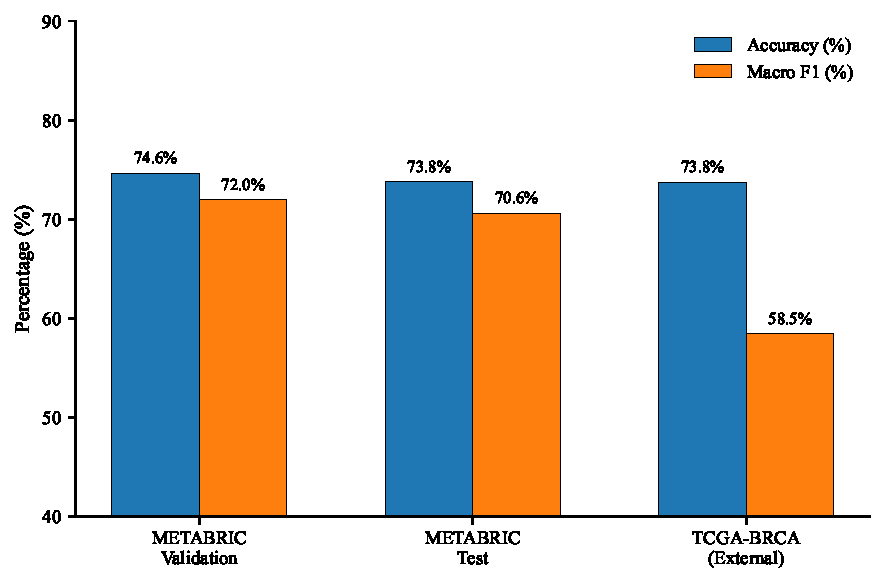
\includegraphics[width=0.72\textwidth]{figures/fig6_cross_platform.pdf}
\caption{Accuracy and macro F1 for the same mRNA-only estimator across METABRIC validation,
METABRIC test, and TCGA-BRCA. TCGA accuracy is similar to the internal estimates, while the
six-class macro F1 is affected by the absent claudin-low class.}
\label{fig:cross_platform}
\end{figure}

\subsubsection{Unlabelled Predictions Did Not Recover the Label Space}

We tested whether the absent class could be detected without annotation-space information.
Unconstrained EM and two detector procedures did not reliably identify it in the tested settings.
\emph{The detection-F1 figures quoted in this and the following two subsections come from the
original scoring function, which returns zero when a detector correctly predicts the empty set;
every cohort with no absent class was therefore scored as a total failure irrespective of the
detector's answer. Section~\ref{sec:detector_v2} re-scores the same simulation under the standard
empty-set convention and should be read as the reference for detector ranking.}

Running the same EM procedure without the mask (em\_full), using the same classifier and
unlabelled target predictions, leaves claudin-low with an estimated
prior of \textbf{0.0751} on TCGA-BRCA and 0.0719 on GSE21653, against a true prevalence of
exactly 0. EM has no signal with which to push that mass to zero: a class that is absent from the
label space still receives probabilistic predictions, and those predictions are
indistinguishable from genuine low-confidence assignments to a rare class. The result is that
em\_full recovers only 2.2 of the 6.9 available points on TCGA-BRCA and leaves macro F1
essentially unchanged (0.585 $\rightarrow$ 0.586), whereas the masked version, given one bit of
annotation knowledge, recovers 6.9 points. We stress that the two runs differ in nothing else.

In this experiment, the predicted marginal was compatible with both an absent class and a rare
class. These results do not prove that no function of unlabeled predictions can distinguish
those cases under any model. They show that the annotation-space fact was not recovered by the
tested EM procedure and detectors.

\subsubsection{A Calibrated Detector Fails to Recover It}

We did not accept that conclusion without testing the obvious workaround: detect the absent class
geometrically. On the probability simplex, a truly absent class should show a deficit of observed
mass relative to its source-expected mass, and we built the ratio statistic described in
Section~\ref{sec:methods_detector} to exploit exactly that. We calibrated the threshold on null
data, consisting of cohorts with no absent class, at level $\alpha = 0.05$, so that a clean cohort is flagged
at most 5\% of the time. This calibration is what makes the test fair; an uncalibrated threshold
would flag absence everywhere.

The detector fails. The null-calibrated threshold is $\tau^\ast = 1.0349$, against a null maximum
ratio with median 1.0184 and maximum 1.0493. Because the null distribution of the maximum ratio
almost reaches the calibrated threshold, the statistic has almost no power: on the calibration set
precision is 0.257 and recall 0.643 (F1 0.367). In the controlled simulation its mean detection F1
is \textbf{0.047} against \textbf{0.549} for EM. Its performance depended on the baseline. Against
the uncorrected model it helped on average (mean $+3.34$ points over 30 cells) but was not reliable.
Its
worst cell is $-2.77$ points, on a cohort with no absent class (73.98\% $\rightarrow$ 71.22\%),
precisely because $\tau^\ast$ flags absent classes that are not there. Against EM, the procedure it
was built to replace, it does not help at all: it wins outright in 11 cells, loses in 9, ties in
10, and its mean gain is \textbf{$-0.37$ points}.

We also tested a generative model-selection detector described in Section~\ref{sec:methods_lrt}.
It fits the target sample as a Gaussian mixture with source-derived components and selects the
label space that minimises BIC over subsets with zero, one, or two absent classes. The complexity
penalty replaces a hand-set threshold. On 30 null cohorts with every class present,
it selects a non-empty absent set in \textbf{27 of 30 runs (90\%)}, and in 23 of those it claims
\emph{two} absent classes. Its mean detection F1 in simulation is 0.209 against 0.549 for EM, and it
loses to EM on accuracy in \textbf{all 30 of 30} cells, by a mean of 17.6 points. A BIC-style
penalty is not sufficient to make an absent class identifiable.

Both detector procedures produced negative results in the tested settings. The geometric statistic
had low detection performance, while the model-selection procedure produced false positives on
clean cohorts. These findings support specifying the target label space from cohort documentation
rather than relying on the tested detectors.

\subsubsection{A Corrected Metric Reverses the Detector Ranking}
\label{sec:detector_v2}

The detector comparison above used a scoring function that returns $0.0$ whenever a detector
correctly predicts the empty set, because the F1 numerator and denominator both vanish. Every
cohort with no absent class was therefore scored as a total failure regardless of whether the
detector was right. Under the standard empty-set convention the comparison changes substantially,
so we re-ran the simulation scoring each cell with micro precision, recall, and exact-set match,
over 20 seeds per cell, six absent sets, three covariate-shift levels, and with and without a
Dirichlet prior shift, giving 36 simulated conditions and 720 evaluated cohorts. The raw detected
and true sets were written to disk so the scoring can be re-examined without re-running the
simulation.

Table~\ref{tab:detector_v2} gives the pooled result across all 720 cohorts. The uncalibrated EM
rule that the paper reported as failing is in fact the strongest of the six on F1 and exact-set
match: its F1 is 0.786 and its exact-set-match rate 0.550, both above every calibrated alternative. The
multiplicity-controlled replacement, which resamples source validation predictions to build a null
and applies Benjamini--Hochberg at $\alpha = 0.05$, is markedly more aggressive: micro precision
falls to 0.577 and it flags a non-empty absent set on 73 of the 120 clean cohorts. The
probability-frequency rule is worse still, flagging 87 of 120. Importance weighting the null by a
discriminator-estimated density ratio reduces the clean-cohort errors to 56 of 120 but also halves
recall, so the correction buys specificity at a real cost in power. Simply declaring a class absent
because the model never predicts it attains perfect precision and an exact-match rate of 0.167 by
predicting nothing, which is the degenerate solution the empty-set convention is designed to expose
rather than reward.

\begin{table}[H]
\centering
\caption{Absent-class detectors scored with the standard empty-set convention
(20 seeds $\times$ 6 absent sets $\times$ 3 covariate-shift levels $\times$ 2 prior-shift settings
$=$ 720 cohorts). Null false positives count cohorts with no absent class on which the detector
returned a non-empty set. The na\"ive rule's perfect precision is
degenerate; its exact-match rate of 0.167 is the fraction of conditions in which nothing was in fact absent.}
\label{tab:detector_v2}
\begin{tabular}{lccccc}
\toprule
\textbf{Detector} & \textbf{Micro P} & \textbf{Micro R} & \textbf{Micro F1} &
\textbf{Exact match} & \textbf{Null FP} \\
\midrule
Uncalibrated EM (\texttt{em\_orig})        & \textbf{0.920} & 0.685 & \textbf{0.786} & \textbf{0.550} & 17/120 \\
Calibrated EM (\texttt{em\_cal})           & 0.577 & \textbf{0.876} & 0.696 & 0.362 & 73/120 \\
Importance-weighted EM (\texttt{em\_cal\_iw}) & 0.540 & 0.544 & 0.542 & 0.242 & 56/120 \\
Probability frequency (\texttt{pfreq})     & 0.548 & 0.902 & 0.682 & 0.372 & 87/120 \\
Geometric coherence (\texttt{geo})         & 0.467 & 0.154 & 0.232 & 0.193 & 27/120 \\
Never predicted (\texttt{naive})           & 1.000 & 0.006 & 0.012 & 0.167 & \textbf{0/120} \\
\bottomrule
\end{tabular}
\end{table}

The pooled figures conceal the structure that matters, which is that detection degrades with
covariate shift and fails differently under prior shift. Restricting to cohorts with a truly absent
class, the uncalibrated rule's mean F1 is 0.995 with no covariate shift and no prior shift, falling
to 0.543 at the highest covariate-shift level with prior shift present. The calibrated detectors
lose control of the clean-cohort error rate when prior shift is present. With no prior shift the
uncalibrated rule flags none of the 20 clean cohorts at any covariate-shift level (0/20), while
\texttt{em\_cal} flags 3, 2, and 11 of 20 and \texttt{pfreq} flags 11, 9, and 7 of 20 as the
covariate shift rises from 0.0 to 0.8. Under prior shift the uncalibrated rule still flags only 9,
3, and 5 of 20, but \texttt{pfreq} flags all 20 clean cohorts at every covariate-shift level and
\texttt{em\_cal} flags 20, 18, and 19 of 20. No detector in the comparison is simultaneously
high-recall and low-false-positive across the two shift axes.

The practical conclusion is unchanged but now rests on a corrected measurement rather than a
metric artefact. Absence of a class is not identifiable from unlabelled predictions by any of the
tested procedures once covariate and prior shift are both present, and the apparent failure of the
original rule was overstated: it is the strongest of the detectors tested on F1 and exact-set
match, and its calibrated replacements trade that strength for clean-cohort false positives. Together with the
EM prior estimate of 0.0751 for an absent class, this supports declaring the target label space
from cohort documentation rather than inferring it.

\subsubsection{Separating Label-Space Mismatch from Prior Shift}

Because the real cohorts change both prevalence and label space simultaneously, we simulated the
two factors independently: label-space mismatch $n_{\text{absent}} \in \{0,1,2\}$, covariate
shift, and prior shift, 20 seeds per cell, $n_{\text{target}} = 1000$
(Section~\ref{sec:methods_sim}). The separation is clean. With \emph{no} prior shift the
correction is worth $-0.4$ to $+3.2$ points, straddling zero and growing only with the number of
absent classes: with no prior shift the label-space term alone contributes roughly $+0.7$ to
$+3.2$ points. With prior shift the correction is worth $+5.9$ to $+7.9$ points in every cell.
The mechanism is that label-space mismatch creates \emph{apparent} prior shift on the remaining
classes. EM can only redistribute mass within the supplied label space, so the two effects can
interact in real cohorts.

The simulation also reproduces the identifiability failure at scale: the oracle-mask column
matches the detected column only when the mask is supplied, and the unguided detector's accuracy
tracks the uncorrected baseline once the absent class is rare.

\subsubsection{Stability of the Correction}

The correction does not depend on how the target is partitioned. Splitting TCGA-BRCA in half and
applying the procedure transductively within each half gives 80.97\% and 80.12\%, a spread of
0.85 points compared with the recovered gain of 6.89. A paired bootstrap over target samples
($n_{\text{iter}} = 2000$) gives a mean gain of \textbf{+6.88 points}, 95\% CI
\textbf{[+4.96, +8.81]}, with $P(\text{gain} > 0) = 1.0$. The gain is therefore not an artifact
of a favourable partition or of a few influential samples.

\begin{figure}[htbp]
\centering
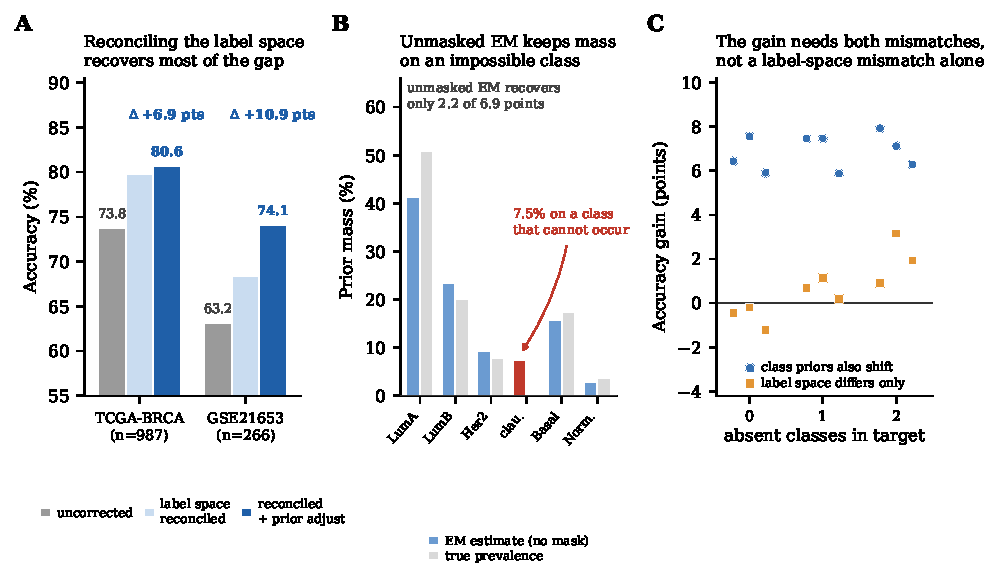
\includegraphics[width=0.95\textwidth]{figures/figH_label_shift.pdf}
\caption{Label-space reconciliation and prior correction. \textbf{(A)} Accuracy before and
after label-space reconciliation on TCGA-BRCA and GSE21653, showing the mask-only and
EM-corrected stages separately. \textbf{(B)} The identifiability failure: unconstrained EM
retains substantial prior mass on claudin-low, whose true prevalence in both cohorts is zero,
and recovers only a fraction of the available gain. \textbf{(C)} Controlled simulation
separating label-space mismatch from prior shift; the correction is near zero without prior shift
and consistently large with it.}
\label{fig:label_shift}
\end{figure}

\subsection{Survival Analysis Validates Prognostic Stratification}
\label{sec:survival}

Cox proportional hazards regression on the METABRIC validation + test sets (n=411, 267 death events, 65\% event rate) confirmed that predicted subtype probabilities carry significant prognostic information. The overall C-Index was 0.598 (log-rank $p = 0.0008$), with time-dependent C-Indices of 0.651 (3-year), 0.622 (5-year), and 0.610 (10-year).

\begin{table}[H]
\centering
\caption{Cox regression hazard ratios for predicted subtypes (Luminal A = reference) on METABRIC (n=411).}
\label{tab:cox}
\begin{tabular}{lccc}
\toprule
\textbf{Predicted Subtype} & \textbf{HR} & \textbf{95\% CI} & \textbf{p-value} \\
\midrule
Luminal B & 1.50 & [1.14, 1.97] & $<0.005$ \\
HER2-enriched & 1.43 & [1.08, 1.89] & 0.01 \\
Basal-like & 1.46 & [1.07, 1.99] & 0.02 \\
Claudin-low & 0.82 & [0.58, 1.16] & 0.25 \\
Normal-like & 1.31 & [0.86, 2.00] & 0.21 \\
\bottomrule
\end{tabular}
\end{table}

On the TCGA-BRCA cohort (n=966, 133 events), the C-Index was 0.577 ($p = 0.047$), with time-dependent C-Indices of 0.587 (3-year), 0.574 (5-year), and 0.577 (10-year). The concordant survival discrimination across both cohorts supports the clinical relevance of the predicted subtypes. The risk score is a Cox model fit on METABRIC training predictions and applied unchanged to TCGA, which requires no outcome information from the validation cohort and is therefore fully reproducible from the released code. An earlier iteration of this analysis reported a C-index of 0.586 ($p = 0.013$) under a variant risk-score construction whose exact form was not retained; because that construction cannot be reconstructed from the preserved pipeline, we report the reproducible figures throughout rather than mixing the two.

\subsection{SHAP Analysis Reveals Modality Contributions}
\label{sec:shap}

SHAP interpretability analysis (Figure~\ref{fig:shap}) quantified the relative importance of each modality. mRNA expression contributed 63.3\% of the model's decisions, followed by methylation (26.7\%) and clinical features (10.0\%). Copy number and mutation data contributed $<$1\% each, consistent with their noise-inducing effect observed in the ablation study.

The top discriminating features included ER/HER2 clinical markers and proliferation features.
Leading mRNA features included \textit{ACP7}, \textit{ACTG2}, \textit{ADIRF}, and \textit{ACOT4}.
These features align with established breast cancer biology and PAM50 subtype definitions.

\begin{figure}[htbp]
\centering
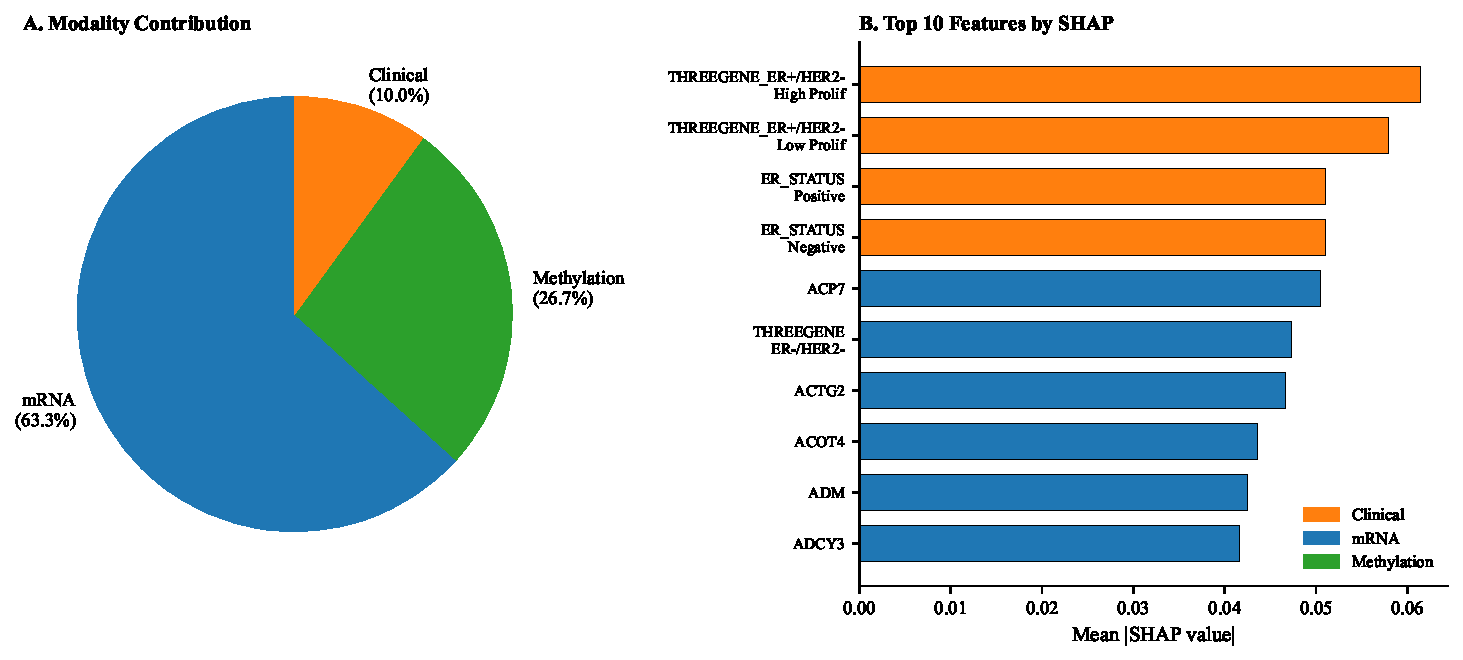
\includegraphics[width=0.85\textwidth]{figures/fig4_shap_analysis.pdf}
\caption{SHAP-based modality attribution. mRNA expression accounts for 63.3\% of model decisions, methylation 26.7\% and clinical features 10.0\%; copy-number and mutation blocks contribute under 1\% each.}
\label{fig:shap}
\end{figure}

\subsection{The Genomic Panel Outperforms Subtype Alone in Treated Subgroups}
\label{sec:route_a_treatment}

We also asked whether the 713-dimension panel adds information beyond the subtype call
itself for clinically relevant stratified outcomes. We defined a 5-year outcome (death within
60 months versus survival beyond it, censored observations excluded) and evaluated within
treatment subgroups, using the same 5-fold protocol and reporting AUC against a PAM50
subtype-only baseline trained on the identical splits.

A necessary caveat: METABRIC's treatment fields record whether a therapy was \emph{administered},
not whether the patient responded. There is no response variable in this dataset, so this is
\emph{prognosis among treated patients}, not treatment-response prediction, and we label it as
such throughout.

\begin{table}[H]
\centering
\caption{5-year outcome discrimination within treatment subgroups, genomic panel versus
PAM50 subtype alone. These are administered-treatment cohorts, not response assessments.}
\label{tab:treatment}
\begin{tabular}{lccccc}
\toprule
\textbf{Treated subgroup} & \textbf{n} & \textbf{Events} & \textbf{AUC (panel)} & \textbf{AUC (subtype)} & \textbf{$\Delta$} \\
\midrule
Chemotherapy & 275 & 120 & 0.624 & 0.571 & $+0.053$ \\
Hormone therapy & 768 & 210 & 0.679 & 0.577 & $+0.102$ \\
Radiotherapy & 767 & 225 & 0.718 & 0.640 & $+0.078$ \\
\bottomrule
\end{tabular}
\end{table}

The panel out-discriminates the subtype-only baseline in all three subgroups
(Figure~\ref{fig:treatment}), with the largest margin in the hormone-therapy cohort
($+0.102$). Because a subtype-only baseline already encodes the dominant prognostic axis, an
increment of this size is consistent with additional prognostic information in within-subtype
expression and methylation variation. This comparison favours the panel over the subtype-only
baseline for risk stratification in these METABRIC treatment subgroups and does not depend on
the Transformer.

\begin{figure}[htbp]
\centering
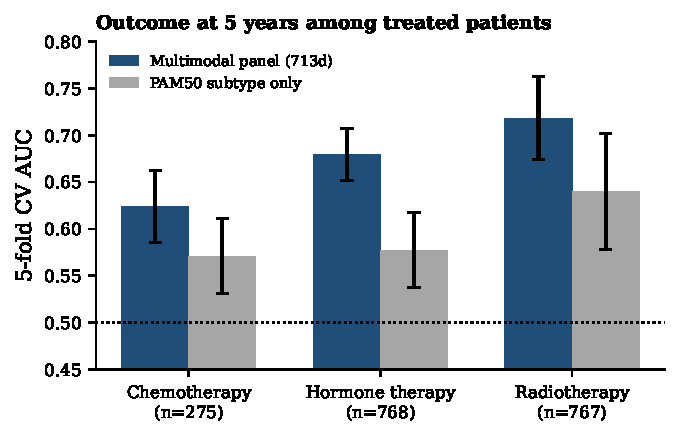
\includegraphics[width=0.72\textwidth]{figures/figF_treatment_auc.pdf}
\caption{Five-year outcome discrimination within treatment subgroups on METABRIC. The
multimodal panel exceeds the PAM50 subtype-only baseline in all three cohorts, most strongly
under hormone therapy.}
\label{fig:treatment}
\end{figure}

\subsection{Treatment-Response Prediction: Subtype Probabilities Track pCR, Genomic Features Add Nothing}
\label{sec:pcr}

Subtype accuracy is a surrogate endpoint. To test whether the framework carries clinical value we
applied it to a genuine response endpoint: pathological complete response (pCR) after neoadjuvant
chemotherapy in GSE20194 (n=278, 56 pCR / 222 residual disease, Affymetrix HG-U133A). The 412-gene
panel covers 276 genes on this platform (67.0\%). We compared a clinical-only model
(age, ER, PR, HER2, grade, histology) against the same model augmented with genomic features and
with predicted subtype probabilities.

The genomic panel did not significantly improve on clinical features in this cohort. Clinical-only
AUC was 0.791, genomic-only AUC was 0.773, and combined AUC was 0.794. The difference was
\textbf{+0.0045} (95\% CI \textbf{[$-0.060$, $+0.061$]}, $P(\Delta > 0) = 0.576$). Adding
predicted subtype probabilities to the clinical model gave an AUC of 0.797, a difference of
$+0.0034$ (95\% CI [$-0.023$, $+0.030$]). Neither increment was distinguishable from zero.
The genomic-only model had lower AUC than the clinical-only model.

What the predictions do capture is biology. Grouping patients by predicted subtype gives pCR rates
that followed the observed subtype pattern: HER2-enriched 53.6\% (15/28), Basal-like 42.4\%
(14/33), claudin-low 26.2\% (11/42), Luminal B 13.2\% (9/68), Luminal A 6.0\% (6/100),
Normal-like 14.3\% (1/7). HER2-enriched and Basal-like had higher observed pCR rates than Luminal A.
The Luminal A estimate is based on 100 patients. Predicted-subtype probabilities alone reached AUC 0.759,
comparable to ER status alone (0.727).

We report this as a negative result. In this cohort, the genomic panel did not improve pCR
prediction beyond routine clinical variables, including receptor status and grade. Its observed
value in this study was prognostic rather than predictive. This is consistent with the related
analysis in
Section~\ref{sec:route_a_treatment}, where the panel out-discriminates a subtype-only baseline for
\emph{outcome} within treated subgroups while METABRIC records treatment administration rather
than response.

\begin{figure}[htbp]
\centering
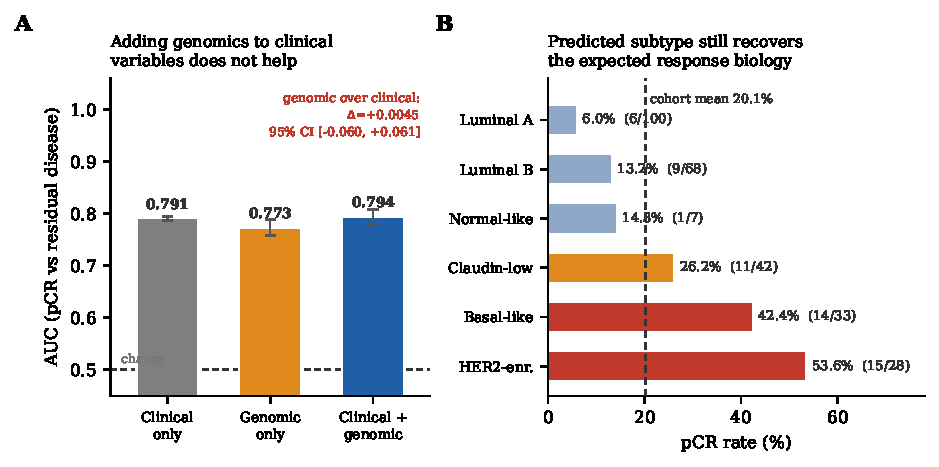
\includegraphics[width=0.95\textwidth]{figures/figI_pcr.pdf}
\caption{Treatment-response prediction in GSE20194 (n=278; 56 pCR, 222 residual disease).
\textbf{(A)} Discrimination of pCR after neoadjuvant chemotherapy. The genomic panel does not
improve on clinical variables: the increment is $+0.0045$ with a 95\% CI spanning zero, and the
genomic-only model (0.773) is worse than clinical-only (0.791). \textbf{(B)} pCR rate by predicted
subtype. Despite adding no predictive value over clinical features, the predicted subtype
reproduces the observed response pattern, with pCR rates of 53.6\% for HER2-enriched and 42.4\%
for basal-like compared with 6.0\% for Luminal A.}
\label{fig:pcr}
\end{figure}


% ============================================================
\section{Methodological Investigation: A Fusion Transformer Does Not Improve PAM50 Prediction}
\label{sec:route_a}

The preceding results establish a linear reference: multinomial logistic regression over
clinical, mRNA and methylation features, reaching 75.3\% cross-validated accuracy. We tested
whether a multimodal fusion architecture could exceed it. The architecture projects each
modality into a shared space and combines them through cross-modal attention. Capacity,
regularization, pretraining, and external-validation experiments produced a negative result.

\subsection{The Gap Is Bias-Limited, Not Optimization-Limited}
\label{sec:route_a_bias}

We swept model capacity across 12 configurations (embedding dimension $d \in \{32,64,128,256\}$
crossed with encoder depth $L \in \{1,2,4\}$), training each with early stopping under the same
5-fold protocol used for the linear reference. All twelve land in a narrow band between 65.5\%
and 69.8\% (Figure~\ref{fig:capacity}), with the best configuration at $d{=}128$, $L{=}4$.
Its accuracy was 5.5 percentage points below the linear reference. Eleven of
twelve configurations cluster within 4 points of one another, so capacity is not the binding
constraint; adding parameters does not move the model toward the reference.

A learning curve on the best small configuration (Figure~\ref{fig:learning}) is still rising but
decelerating: 62.2\%, 64.7\%, 66.5\% and 68.0\% at $n = 240, 479, 718$ and 958 training samples.
The marginal return is 0.43 accuracy points per additional 100 samples. Fitting
$\mathrm{acc}(n) = a + b\ln n$ gives $a = 39.6$, $b = 4.10$, which projects that
The fitted curve projects that \textbf{5{,}939 samples}, 6.2 times the current training set,
would be required to reach parity with logistic regression. It projects 11{,}579 samples for 78\%.

Taken together these two experiments indicate a bias limitation rather than a variance
limitation. A variance problem is fixed by more data or stronger regularization; a bias problem
is fixed by changing the hypothesis class. Since the architecture's irreducible performance sits
below the linear model's, our working conclusion is that cross-modal attention is simply a
poorer inductive bias than a linear combination on this problem, where 713 features describe
958 patients and the signal-to-noise ratio in the copy-number and mutation blocks is low.

\subsection{Regularization Does Not Close the Gap}
\label{sec:route_a_reg}

If the deficit were variance, regularization would recover it. We swept five axes: modality-level
dropout (a per-modality Bernoulli gate), weight decay, label smoothing, feature dropout, and
reduced width combined with depth (Figure~\ref{fig:regularization}). The strongest single axis,
modality dropout at 0.2, moves the baseline from 67.7\% to 68.6\%, a gain of 0.84 points. The
best two-axis combination (modality dropout 0.2 with weight decay 0.05) reaches 68.1\%, no better
than the best single axis. Every configuration remains roughly 7 points below the reference,
which corroborates the bias reading: the deficit is not recoverable by constraining the
optimizer's search.

\subsection{Self-Supervised Pretraining Helps Internally but Not Externally}
\label{sec:route_a_pretrain}

The one intervention that produced a real internal gain was self-supervised pretraining.
Following the earlier autoencoder work, we pretrained the modality encoders with a
masked-feature reconstruction objective: a random 30\% of features in each modality are zeroed
and the modality token must reconstruct them through a linear decoder. To keep the estimate
honest, the encoder is pretrained \emph{separately within each cross-validation fold}, on that
fold's training portion only; pretraining once on the full dataset before splitting would leak
information and inflate the score.

Pretraining raised cross-validated accuracy from 67.3\% to 70.0\%, a gain of 2.7 points
 (Figure~\ref{fig:pretraining}). This was the best result any Transformer variant achieved in
the study and exceeded the gain from any individual regularization axis. The gain did not survive external
validation.

\subsection{External Validation Reverses the Ranking}
\label{sec:route_a_tcga}

We evaluated all three models on TCGA-BRCA (n=987) using the within-platform rank normalization
adopted earlier, and additionally carried each model through to a survival C-index (Cox model
fitted on METABRIC predictions, applied unchanged to TCGA; nothing is fitted on TCGA).

The linear reference reached 73.8\% accuracy. The unguided Transformer reached 66.1\%.
These results use the 412-gene mRNA panel. The pretrained Transformer, which had the best internal
cross-validation score, fell to 62.7\%, \emph{worse} than the unguided model
(Figure~\ref{fig:route_a_tcga}). Its internal-to-external drop is 7.3 points, compared with 1.2
points for the unguided Transformer and 1.5 points for the linear reference. The external survival
C-indices show the same ordering: 0.577 (linear), 0.551 (Transformer), 0.530 (pretrained
Transformer).

\begin{table}[H]
\centering
\caption{Internal versus external performance for the mRNA-only reference and two Transformer
variants using the 412-gene panel. All models were evaluated on TCGA with the same
within-platform rank-normalization protocol.}
\label{tab:route_a}
\begin{tabular}{lccc}
\toprule
\textbf{Model} & \textbf{METABRIC CV} & \textbf{TCGA accuracy} & \textbf{TCGA C-index} \\
\midrule
Logistic regression (reference) & 75.3\% & 73.8\% & 0.577 \\
Fusion Transformer & 67.3\% & 66.1\% & 0.551 \\
\quad + pretraining & \textbf{70.0\%} & 62.7\% & 0.530 \\
\bottomrule
\end{tabular}
\end{table}

This reversal is the central methodological finding. Pretraining on METABRIC's masked-feature
distribution teaches the encoder to exploit covariance structure specific to that cohort;
the encoder becomes a better METABRIC model, not a better model of breast cancer. Under
cross-validation the effect looks like genuine improvement, because the held-out fold is drawn
from the same distribution. Only external validation distinguishes the two interpretations. An
internal gain of 2.7 points accompanied by an external loss of 3.4 points is a signature of
cohort-specific overfitting, and it is the reason we report the Transformer as a negative
result rather than as the paper's method.

\subsection{A Second External Cohort Confirms the Augmented Model Does Not Transfer}
\label{sec:route_a_gse}

To test whether the Transformer's deficit was an artifact of validating on a single platform,
we assembled a second external cohort from GEO. GSE21653 (n=266, Affymetrix U133 Plus 2.0)
carries PAM50 molecular-subtype calls and DFS time/event for every sample. It is a harder
cohort than TCGA: basal-like tumours make up 28\% of it against 17\% in TCGA, and it contains
no claudin-low annotations. Of the 412 panel genes, 369 (89.6\%) map to a GPL570 probe; where
several probes map to one gene we retain the highest-mean probe, a fixed rule that uses no
label information.

Under the identical rank-normalization protocol, the linear reference reached 63.2\% accuracy
(macro F1 0.504). We also retrained the reference on the same 369 genes and evaluated it on
TCGA, where it reached 74.6\%. This comparison holds the feature set and training data
constant, but other cohort differences remain and cannot be attributed to composition alone.
The external survival C-index was 0.584 (log-rank $p=0.011$, n=252, 83 events). This estimate
was similar to TCGA (0.577), which is the useful
observation: the model's \emph{discrimination} transfers across two distinct expression
platforms even though its absolute classification accuracy is much lower on the
basal-enriched cohort. The drop is not uniform across subtypes. It is concentrated in the basal-like class, which
rises from 10.4\% of the training set to 28.2\% of this cohort and accounts for 29 of the 98
errors (30\%) despite a precision of 0.98: almost every sample predicted basal-like is one,
but only 61\% of true basal-like samples are recovered, against 77\% recall on the same class
in TCGA. Normal-like is the other weak class (recall 0.345 on 29 samples). Discrimination on
well-represented classes is preserved (Luminal A recall 0.775), and the unweighted per-class
accuracy is 0.578 against a raw 0.632. This pattern is consistent with a class-prior shift
acting on a decision boundary calibrated to METABRIC's composition rather than with a failure
of the learned representation, and it is a limitation that prior-probability recalibration or
cohort-specific class weights would plausibly address.

\subsection{Additional Training Data Narrows the Gap Exactly as Predicted}
\label{sec:route_a_multicohort}

The diagnosis in Section~\ref{sec:route_a_bias} made a falsifiable prediction: the Transformer
is data-limited, and its accuracy should rise along the fitted learning curve as samples are
added. GSE21653 provides a direct test. Pooling it with METABRIC gives 1{,}224 training samples,
28\% more than the original 958, and we evaluate on TCGA so the external endpoint is unchanged.

\begin{table}[H]
\centering
\caption{Effect of adding GSE21653 to training, evaluated on TCGA (n=987) using the 369 genes
shared across METABRIC, GSE21653, and TCGA. These results use a different feature set from the
412-gene comparison in Table~\ref{tab:route_a}.}
\label{tab:multicohort}
\begin{tabular}{lccc}
\toprule
\textbf{Model} & \textbf{METABRIC only} & \textbf{+ GSE21653} & \textbf{$\Delta$} \\
\midrule
Logistic regression & 74.6\% & 73.6\% & $-1.01$ \\
Fusion Transformer & 64.8\% & 66.0\% & $+1.11$ \\
\quad + pretraining & 65.7\% & 64.7\% & $-0.91$ \\
\bottomrule
\end{tabular}
\end{table}

Adding a second cohort raised the unguided Transformer by 1.11 points. The learning-curve
prediction was $4.10 \times \ln(1224/958) = 1.00$ point, a difference of 0.11 points. The
model sits close to its extrapolated trajectory, which is consistent with the deficit being a
bias limitation: the architecture is learning what it can from the available signal, and more
data helps it at precisely the rate the curve implies.
The Transformer-versus-linear gap narrows from 9.7 to 7.6 points but remains large; closing it
by data alone would require roughly six times the present training set.

Two secondary observations reinforce the picture. The linear reference \emph{lost} 1.01 points
from the additional cohort, and the pretrained model lost 0.91 points. Models that fit
cohort-specific structure tightly are the ones harmed by a heterogeneous training mixture,
whereas the unguided Transformer was underfitting and benefited from more data. This is the same
bias--variance story from the opposite direction, and it is another reason we prefer the linear
reference for this task while reporting the Transformer's behaviour honestly.

% ============================================================
\section{Discussion}
\label{sec:discussion}

Our primary contribution is an empirical analysis of how annotation-space differences affect
cross-cohort evaluation of breast cancer molecular-subtype classifiers. We do not propose a new
label-shift estimator. Instead, we show that applying an externally specified PAM50 label space
changes reported scores for two cohorts, and that this operation must be distinguished from
improving the classifier itself.

\textbf{The effect depends on the metric and cohort.} TCGA-BRCA accuracy (73.76\%) was nearly
identical to METABRIC test accuracy (73.8\%), so these data do not show an accuracy transfer gap
for TCGA before reconciliation. However, six-class macro F1 on TCGA was 0.585, compared with
0.702 when averaged over its five annotated classes. On GSE21653, baseline accuracy was 63.16\%,
and the combined PAM50 restriction plus EM correction yielded 74.06\%. These observations support
a narrower conclusion: cross-cohort metrics can change when the evaluation label space is
reconciled, while residual differences may also reflect platform, prevalence, sample composition,
or other cohort effects.

\textbf{The tested procedures did not recover the label space from unlabeled predictions.}
Unconstrained EM retained an estimated prior of 0.0751 for claudin-low on TCGA-BRCA, although
that class is absent under PAM50 annotation. The geometric detector had low simulated detection
F1 under both scorings ($0.047$ originally, $0.232$ under the standard empty-set convention),
and the BIC procedure selected a non-empty absent set in 90\% of clean null runs; the
uncalibrated EM rule that ranked best of the six after re-scoring still flags clean cohorts
once prior shift is present.
These results show that the tested procedures did not reliably identify the annotation space at
these sample sizes. They do not establish a general impossibility theorem for every classifier
or detector. In practice, the allowed target labels should be specified from cohort documentation,
rather than inferred from these predictions alone.

\textbf{Separating label-space and prior changes matters.} In the controlled simulation, the
correction changed accuracy by $-0.4$ to $+3.2$ points without prior shift and by $+5.9$ to
$+7.9$ points when prior shift was also present. These results indicate that the effects can
interact under the tested settings. They should not be read as calibrated estimates for an
unobserved clinical cohort.

\textbf{Modality selection is internal, and the multimodal advantage does not transfer.} The
three-modality model outperformed the five-modality model in the reported METABRIC split and
cross-validation. Section~\ref{sec:external_multimodal} tests whether that advantage survives
external validation, in a reduced three-layer space that both METABRIC and TCGA-BRCA carry.
It does not. Adding methylation is flat internally and lowers external accuracy by 1.9 points;
the harmonized clinical block raises internal cross-validated and held-out scores but moves
external accuracy by 0.3 points or less, with all multimodal-versus-mRNA comparisons
non-significant ($p = 0.13$ to $1.00$). The internal blocks that help most are precisely the
ones that cannot be transported: the original 713-dimension flagship reaches 75.92\% internally
against 73.17\% for the harmonized tri-modal model, and the 2.75-point difference is
contributed by METABRIC-specific clinical fields (NPI, GRADE, INTCLUST, THREEGENE, cohort
indicator) that have no counterpart in the target cohort. Low SHAP attribution for copy-number
and mutation features is consistent with limited contribution in this fitted model, but does
not establish that these modalities are uninformative in other cohorts or models. We therefore
report the multimodal result as internal and do not claim transportable multimodal gain.

\textbf{Rank normalization handles the feature side; it does not handle the label side.} The
within-platform rank normalization strategy transfers the feature distribution across platforms
without retraining: with it, TCGA-BRCA holds its METABRIC accuracy despite the shift from
microarray to RNA-seq, whereas METABRIC-statistic standardization collapses it to 20.7\%. That
result is real but partial, and our analysis shows why. Normalization operates on features and is
therefore blind to a mismatched label space; the two failures are orthogonal and require
different remedies. What transfers most cleanly across all three cohorts is the survival risk
signal (C-index 0.577 and 0.584 on the external cohorts, against 0.598 internally), because
discrimination of risk does not depend on the class label being well-calibrated to a local
annotation standard. Practically, we would deploy the rank-normalized model with an explicit
per-cohort label-space declaration, and treat survival discrimination rather than subtype
accuracy as the more portable endpoint.

\textbf{Luminal A/B confusion.} Confusion between Luminal A and Luminal B subtypes is a known challenge \citep{bastien2012pam50}. These subtypes share ER-positive status and differ primarily in proliferation-related gene expression. The 24\% Luminal B-to-Luminal A misclassification rate suggests that proliferation-specific markers such as Ki-67 could improve discrimination.

\textbf{Clinical implications.} The significant survival stratification (C-Index 0.598, $p = 0.0008$) demonstrates that the predicted subtypes carry meaningful prognostic information. The Cox regression hazard ratios align with established prognostic rankings: Luminal B, HER2-enriched, and Basal-like subtypes show elevated mortality risk relative to Luminal A \citep{prat2014research}.


\textbf{Attention-based fusion did not improve the tested models.} We tested the
obvious objection to a linear model, namely that it cannot capture interactions between modalities, by
building a cross-modal attention architecture and giving it every reasonable opportunity to
succeed. It did not. Capacity sweeps, learning curves, five regularization axes and
self-supervised pretraining all failed to bring it to parity, and the diagnosis is specific: the
deficit is a bias limitation, not a variance limitation. With 713 features and 958 training
patients, a linear combination is a better-matched hypothesis class than a sequence of attention
blocks in these experiments. The most instructive outcome is the reversal under external
validation: pretraining produced the largest internal gain of any intervention (+2.7 points) and
the largest external loss ($-$3.4 points relative to the unguided model). This is a caution
about how such architectures are evaluated. A cross-validated improvement is not evidence of a
better model of biology when the held-out data are drawn from the same cohort; only external
validation separates a generalizable gain from cohort-specific overfitting. We therefore report
the Transformer as a negative result, and note that the same reasoning weakens any internal-only
claim for deep fusion models in this domain, where cohorts in the low thousands of samples are
the norm.

\textbf{Panel value beyond the subtype call.} Among treated patients, the 713-dimension panel
out-discriminated a PAM50-subtype-only baseline in all three treatment cohorts, most strongly
for hormone therapy ($+0.102$ AUC). Since the subtype call already encodes the dominant
prognostic axis, this increment indicates that within-subtype molecular variation carries
prognostic information the subtype label discards. This is a clinically motivated use of the
panel that does not depend on the Transformer, and it is where the multimodal representation
earns its keep. The finding is bounded by an important caveat: METABRIC records treatment
administration rather than response, so these are prognosis estimates within treated subgroups,
not predictions of therapeutic response. Establishing genuine response prediction would require
a cohort with RECIST-style or pathological-complete-response annotations.

\textbf{Limitations.} First, the model was developed on METABRIC and ancestry-specific performance was not assessed. Second, the label-space analysis covers one absent class, claudin-low, in two PAM50-annotated cohorts. Third, detector results apply to the tested methods and sample sizes; the controlled simulation uses Gaussian-mixture surrogates rather than expression data and is not a forecast for a new cohort. Fourth, the multimodal model was evaluated externally only in a reduced shared space: 59 of its 69 clinical dimensions have no counterpart in the TCGA schema, so the harmonized comparison in Section~\ref{sec:external_multimodal} substitutes a 10-field clinical block and accepts a 2.75-point internal penalty relative to the original model, and the negative result reported there concerns that reduced configuration rather than every possible multimodal design. Finally, the training sample size may constrain nonlinear models, and the SHAP analysis used a linear explainer that may not capture nonlinear feature effects.

% ============================================================
\section{Conclusion}
\label{sec:conclusion}

Our findings show that cross-cohort subtype metrics can depend on whether the evaluation label
space matches the target cohort's annotation standard. Accuracy on TCGA-BRCA was similar to the
METABRIC test accuracy, but the six-class macro F1 included a zero score for the absent
claudin-low class. On GSE21653, restricting predictions to PAM50 classes and applying EM prior
correction increased accuracy from 63.16\% to 74.06\%. These operations change how predictions
are evaluated; they do not improve the classifier's learned representation. The tested
unconstrained EM and absent-class detectors did not reliably recover the target label space from
unlabeled predictions. Cohort comparisons should therefore report the annotation-defined label
space and the metric's class set explicitly.

The multimodal METABRIC model achieved 75.3\% $\pm$ 2.6\% cross-validated accuracy and 73.8\%
test accuracy. Survival discrimination was similar across the two external cohorts (C-index 0.577
and 0.584), and in a reduced three-layer space shared with TCGA-BRCA the internal multimodal
advantage did not transfer: no configuration beat mRNA alone significantly, and the best
internal model depended on 59 METABRIC-specific clinical dimensions. Cross-modal attention fusion did not outperform the linear reference in
the tested experiments, and the internal gain from pretraining did not transfer to TCGA. These
findings are limited to the cohorts, label spaces, and model configurations studied here.

\section*{Declarations}
\textbf{Data availability:} METABRIC and TCGA-BRCA are available through cBioPortal
(\url{https://www.cbioportal.org/}). GEO accession records are available for
\href{https://www.ncbi.nlm.nih.gov/geo/query/acc.cgi?acc=GSE21653}{GSE21653} and
\href{https://www.ncbi.nlm.nih.gov/geo/query/acc.cgi?acc=GSE20194}{GSE20194}. Redistribution of
processed data should follow the terms of the source repositories.

\textbf{Code availability:} The analysis scripts, derived result files, and figure
generators used for the reported results are available at
\href{https://github.com/HAHA12345677888/pam50-label-space}{GitHub} (public
repository, \texttt{main} branch). A versioned archive with a citable DOI will be
deposited before publication.

\textbf{Author contributions:} Shuxing Liu contributed to the study conception, data analysis, and manuscript preparation.

\textbf{Funding:} Funding information has not been provided.

\textbf{Competing interests:} The authors declare no competing interests.

\textbf{Ethics approval and consent to participate:} The analyses use public cohort resources. The analyses were conducted in compliance with institutional review requirements for publicly available datasets.

\textbf{Correspondence:} Correspondence and requests for materials should be addressed to Shuxing Liu (email: liushuxing8888@student.usm.my).

% ============================================================

\begin{figure}[htbp]
\centering
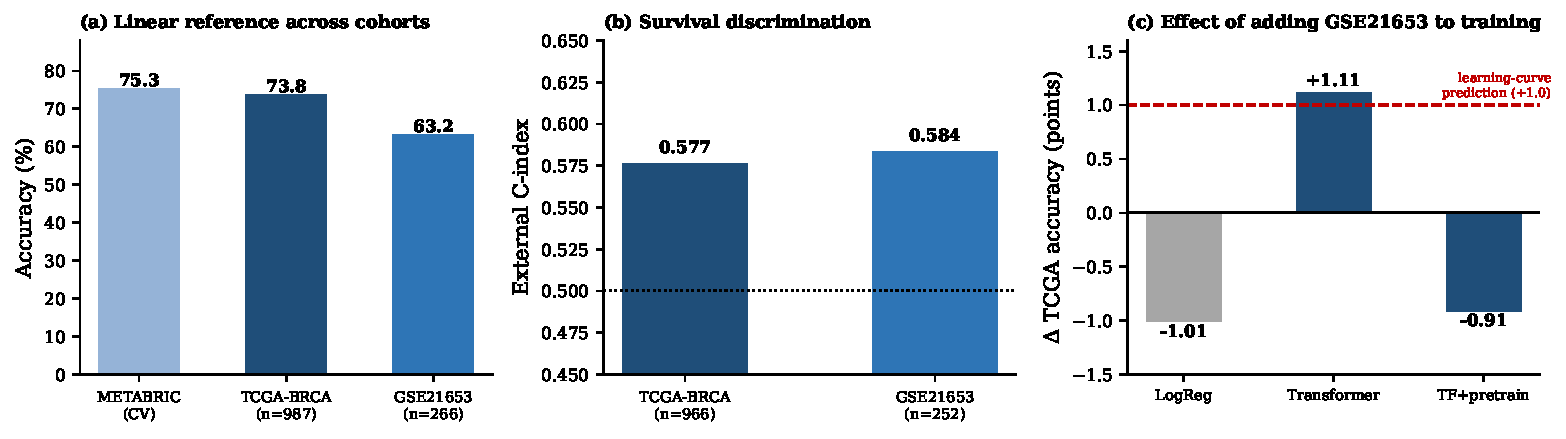
\includegraphics[width=0.98\textwidth]{figures/figG_second_cohort.pdf}
\caption{Second external cohort and the multi-cohort training test. (a) Linear-reference
accuracy across cohorts; (b) external survival C-index on the two independent cohorts, which
agrees closely despite different class composition; (c) change in TCGA accuracy after
GSE21653 is added to training. The unguided Transformer matches its predicted learning-curve
gain, while the linear and pretrained models lose accuracy.}
\label{fig:second_cohort}
\end{figure}

% ---------------- Route A figures ----------------
\begin{figure}[htbp]
\centering
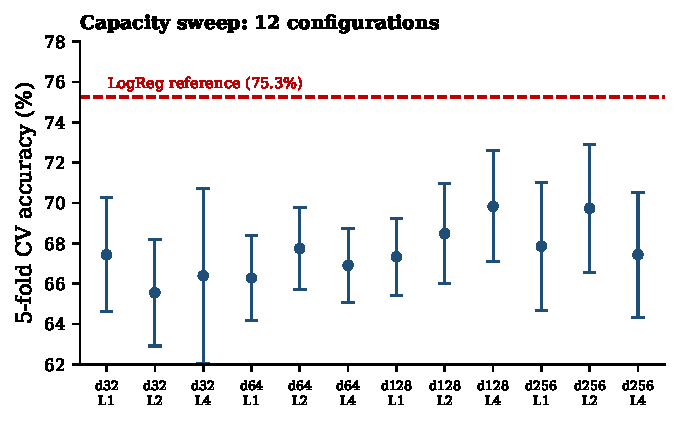
\includegraphics[width=0.8\textwidth]{figures/figB_capacity_sweep.pdf}
\caption{Capacity sweep over 12 configurations ($d \times L$). Every configuration lies below
the logistic-regression reference (dashed), and eleven of twelve fall within a 4-point band,
indicating that capacity is not the binding constraint.}
\label{fig:capacity}
\end{figure}

\begin{figure}[htbp]
\centering
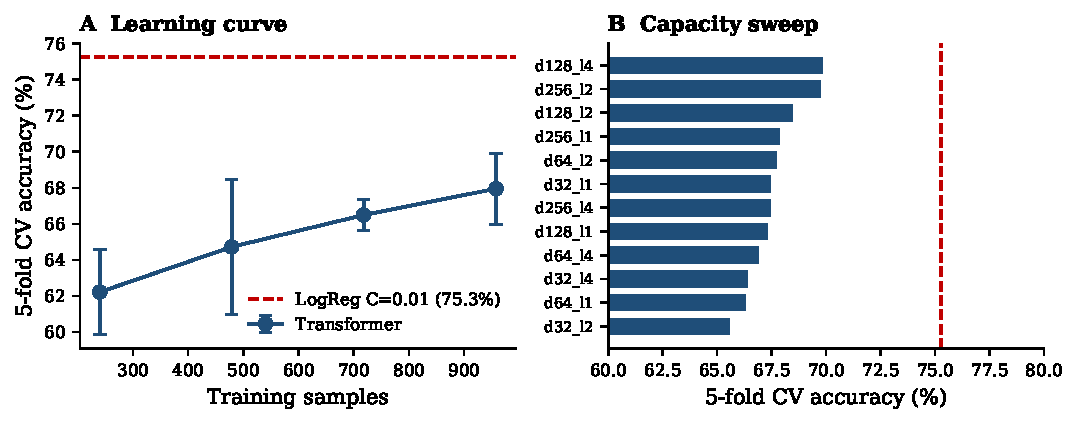
\includegraphics[width=0.8\textwidth]{figures/figA_learning_curves.pdf}
\caption{Learning curve for the best small configuration, with the logistic-regression
reference. The curve is decelerating; extrapolation places parity at roughly six times the
present training set.}
\label{fig:learning}
\end{figure}

\begin{figure}[htbp]
\centering
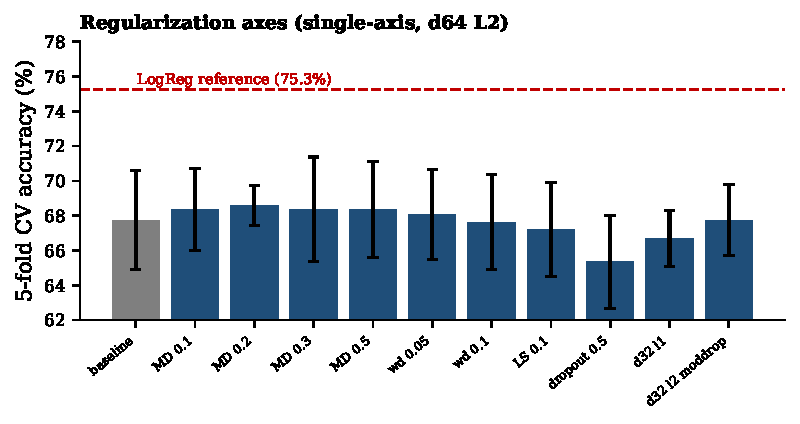
\includegraphics[width=0.8\textwidth]{figures/figC_regularization.pdf}
\caption{Single-axis regularization sweep. The strongest intervention gains 0.84 points, and no
configuration approaches the logistic-regression reference.}
\label{fig:regularization}
\end{figure}

\begin{figure}[htbp]
\centering
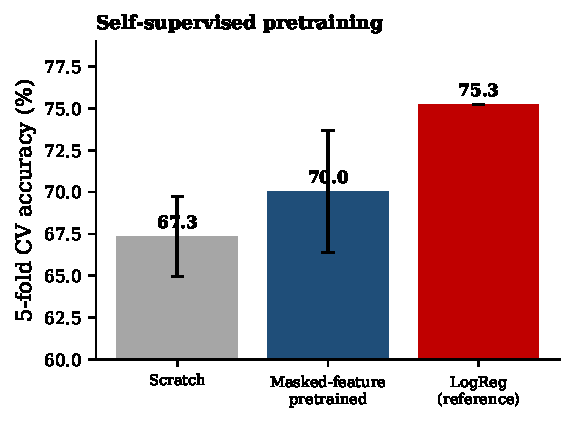
\includegraphics[width=0.55\textwidth]{figures/figD_pretraining.pdf}
\caption{Masked-feature pretraining raises cross-validated accuracy by 2.7 points, the largest
internal gain of any intervention tested, without reaching the linear reference.}
\label{fig:pretraining}
\end{figure}

\begin{figure}[htbp]
\centering
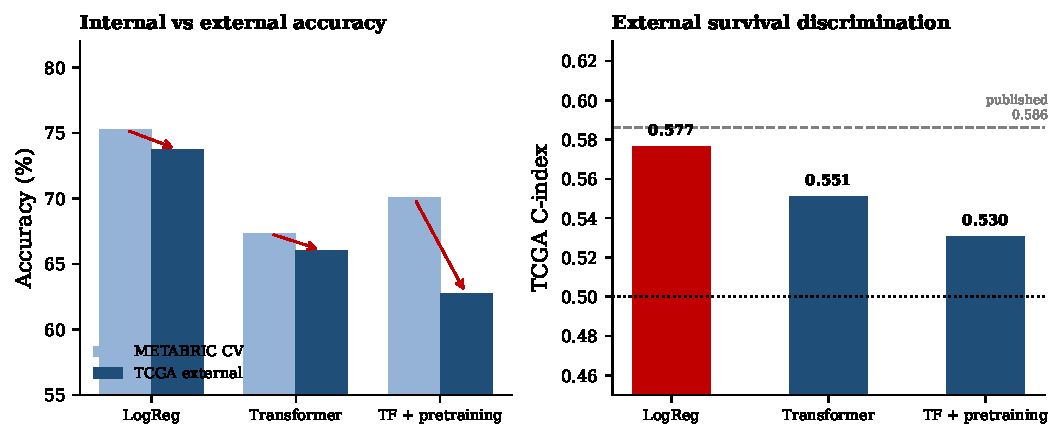
\includegraphics[width=0.95\textwidth]{figures/figE_tcga_validation.pdf}
\caption{Internal versus external performance. Left: accuracy on METABRIC cross-validation and
on TCGA. Right: external survival C-index. The pretrained Transformer shows the largest
internal-to-external drop, and the lowest external C-index.}
\label{fig:route_a_tcga}
\end{figure}

\bibliographystyle{plainnat}
\bibliography{references}

% ============================================================
\end{document}